%Version 3.1 December 2024
% See section 11 of the User Manual for version history
%
%%%%%%%%%%%%%%%%%%%%%%%%%%%%%%%%%%%%%%%%%%%%%%%%%%%%%%%%%%%%%%%%%%%%%%
%%                                                                 %%
%% Please do not use \input{...} to include other tex files.       %%
%% Submit your LaTeX manuscript as one .tex document.              %%
%%                                                                 %%
%% All additional figures and files should be attached             %%
%% separately and not embedded in the \TeX\ document itself.       %%
%%                                                                 %%
%%%%%%%%%%%%%%%%%%%%%%%%%%%%%%%%%%%%%%%%%%%%%%%%%%%%%%%%%%%%%%%%%%%%%

%%\documentclass[referee,sn-basic]{sn-jnl}% referee option is meant for double line spacing

%%=======================================================%%
%% to print line numbers in the margin use lineno option %%
%%=======================================================%%

%%\documentclass[lineno,pdflatex,sn-basic]{sn-jnl}% Basic Springer Nature Reference Style/Chemistry Reference Style

%%=========================================================================================%%
%% the documentclass is set to pdflatex as default. You can delete it if not appropriate.  %%
%%=========================================================================================%%

%%\documentclass[sn-basic]{sn-jnl}% Basic Springer Nature Reference Style/Chemistry Reference Style

%%Note: the following reference styles support Namedate and Numbered referencing. By default the style follows the most common style. To switch between the options you can add or remove “Numbered” in the optional parenthesis. 
%%The option is available for: sn-basic.bst, sn-chicago.bst%  
 
%%\documentclass[pdflatex,sn-nature]{sn-jnl}% Style for submissions to Nature Portfolio journals
%%\documentclass[pdflatex,sn-basic]{sn-jnl}% Basic Springer Nature Reference Style/Chemistry Reference Style
\documentclass[pdflatex,sn-mathphys-num]{sn-jnl}% Math and Physical Sciences Numbered Reference Style
%%\documentclass[pdflatex,sn-mathphys-ay]{sn-jnl}% Math and Physical Sciences Author Year Reference Style
%%\documentclass[pdflatex,sn-aps]{sn-jnl}% American Physical Society (APS) Reference Style
%%\documentclass[pdflatex,sn-vancouver-num]{sn-jnl}% Vancouver Numbered Reference Style
%%\documentclass[pdflatex,sn-vancouver-ay]{sn-jnl}% Vancouver Author Year Reference Style
%%\documentclass[pdflatex,sn-apa]{sn-jnl}% APA Reference Style
%%\documentclass[pdflatex,sn-chicago]{sn-jnl}% Chicago-based Humanities Reference Style

%%%% Standard Packages
%%<additional latex packages if required can be included here>

\usepackage{graphicx}%
\usepackage{multirow}%
\usepackage{amsmath,amssymb,amsfonts}%
\usepackage{amsthm}%
\usepackage{mathrsfs}%
\usepackage[title]{appendix}%
\usepackage{xcolor}%
\usepackage{textcomp}%
\usepackage{manyfoot}%
\usepackage{booktabs}%
\usepackage{algorithm}%
\usepackage{algorithmicx}%
\usepackage{algpseudocode}%
\usepackage{listings}%
\usepackage{tikz}%
\usetikzlibrary{positioning,fit,calc}%
%%%%

%%%%%=============================================================================%%%%
%%%%  Remarks: This template is provided to aid authors with the preparation
%%%%  of original research articles intended for submission to journals published 
%%%%  by Springer Nature. The guidance has been prepared in partnership with 
%%%%  production teams to conform to Springer Nature technical requirements. 
%%%%  Editorial and presentation requirements differ among journal portfolios and 
%%%%  research disciplines. You may find sections in this template are irrelevant 
%%%%  to your work and are empowered to omit any such section if allowed by the 
%%%%  journal you intend to submit to. The submission guidelines and policies 
%%%%  of the journal take precedence. A detailed User Manual is available in the 
%%%%  template package for technical guidance.
%%%%%=============================================================================%%%%

%% as per the requirement new theorem styles can be included as shown below
\theoremstyle{thmstyleone}%
\newtheorem{theorem}{Theorem}%  meant for continuous numbers
%%\newtheorem{theorem}{Theorem}[section]% meant for sectionwise numbers
%% optional argument [theorem] produces theorem numbering sequence instead of independent numbers for Proposition
\newtheorem{proposition}[theorem]{Proposition}% 
%%\newtheorem{proposition}{Proposition}% to get separate numbers for theorem and proposition etc.

\theoremstyle{thmstyletwo}%
\newtheorem{example}{Example}%
\newtheorem{remark}{Remark}%

\theoremstyle{thmstylethree}%
\newtheorem{definition}{Definition}%

\raggedbottom
%%\unnumbered% uncomment this for unnumbered level heads

\begin{document}

\title[Article Title]{Decomposition Approaches for Cross-Domain Recommendation Systems}

%%=============================================================%%
%% GivenName	-> \fnm{Joergen W.}
%% Particle	-> \spfx{van der} -> surname prefix
%% FamilyName	-> \sur{Ploeg}
%% Suffix	-> \sfx{IV}
%% \author*[1,2]{\fnm{Joergen W.} \spfx{van der} \sur{Ploeg} 
%%  \sfx{IV}}\email{iauthor@gmail.com}
%%=============================================================%%
% --- आपका ऑथर ब्लॉक यहाँ से ---

\author[1]{\fnm{Atul} \sur{Patel}}
\email{atulpatel12322@bhu.ac.in}
\equalcont{These authors contributed equally to this work.}

\author*[2]{\fnm{Vibhor} \sur{Kant}}
\email{vibhor.kant@bhu.ac.in}
\equalcont{These authors contributed equally to this work.}

\author[3]{\fnm{Pragya} \sur{Dwivedi}}
\email{pragyadwi86@mnnit.ac.in}


\equalcont{These authors contributed equally to this work.}

% --- Affiliations ---

\affil[1]{\orgdiv{Department of Computer Science, Institute of Science}, \orgname{Banaras Hindu University}, \city{Varanasi}, \postcode{221005}, \state{UP}, \country{India}}

\affil[2]{\orgdiv{Department of Computer Science, Rajiv Gandhi South Campus}, \orgname{Banaras Hindu University}, \city{Mirzapur}, \postcode{231001}, \state{UP}, \country{India}}

\affil[3]{\orgname{Motilal Nehru National Institute of Technology Allahabad}, \city{Prayagraj}, \postcode{211004}, \state{Uttar Pradesh}, \country{India}}
%% Sample for unstructured abstract %%
%%==================================%%

\abstract{Cross-Domain Recommendation Systems (CDRS) mitigate data sparsity in collaborative filtering by transferring knowledge from richer source domains. While the state of the art increasingly relies on complex deep, adversarial, and graph architectures, the comparative behaviour of the underlying classical decomposition operators under controlled sparsity remains under-studied. This paper presents a comparative evaluation---not a new model---of five foundational approaches: Matrix Factorization (MF), Matrix Factorization with Bias (MFB), Non-Negative Matrix Factorization (NMF), Deep Matrix Factorization (DMF), and Singular Value Decomposition (SVD), each adapted to the same two-phase source-to-target protocol. On six Amazon category pairs and four training ratios (20\%--80\%), with MAE/RMSE under five-fold cross-validation, MFB is consistently strongest (MAE typically $0.65$--$0.79$; e.g., $0.6834$ on $CX_1$ at 20\% training versus $0.7637$ for DMF). The comparison indicates that explicit user/item bias modelling is more robust in sparse targets than unconstrained factors, non-negative parts-based factors, or a shallow non-linear interaction, and it offers a practical reference baseline for future CDRS designs.}

%%================================%%
%% Sample for structured abstract %%
%%================================%%

% \abstract{\textbf{Purpose:} The abstract serves both as a general introduction to the topic and as a brief, non-technical summary of the main results and their implications. The abstract must not include subheadings (unless expressly permitted in the journal's Instructions to Authors), equations or citations. As a guide the abstract should not exceed 200 words. Most journals do not set a hard limit however authors are advised to check the author instructions for the journal they are submitting to.
% 
% \textbf{Methods:} The abstract serves both as a general introduction to the topic and as a brief, non-technical summary of the main results and their implications. The abstract must not include subheadings (unless expressly permitted in the journal's Instructions to Authors), equations or citations. As a guide the abstract should not exceed 200 words. Most journals do not set a hard limit however authors are advised to check the author instructions for the journal they are submitting to.
% 
% \textbf{Results:} The abstract serves both as a general introduction to the topic and as a brief, non-technical summary of the main results and their implications. The abstract must not include subheadings (unless expressly permitted in the journal's Instructions to Authors), equations or citations. As a guide the abstract should not exceed 200 words. Most journals do not set a hard limit however authors are advised to check the author instructions for the journal they are submitting to.
% 
% \textbf{Conclusion:} The abstract serves both as a general introduction to the topic and as a brief, non-technical summary of the main results and their implications. The abstract must not include subheadings (unless expressly permitted in the journal's Instructions to Authors), equations or citations. As a guide the abstract should not exceed 200 words. Most journals do not set a hard limit however authors are advised to check the author instructions for the journal they are submitting to.}

\keywords{ Cross-domain recommendation, Data sparsity, Decomposition approaches, Knowledge transfer, Matrix factorization}

%%\pacs[JEL Classification]{D8, H51}

%%\pacs[MSC Classification]{35A01, 65L10, 65L12, 65L20, 65L70}

\maketitle

\section{Introduction}\label{sec1}

Recommender systems are widely used for personalization in e-commerce, entertainment, and social media~\cite{schafer1999recommender, lu2015recommender, resnick1997recommender}. Industry reports attribute about 35\% of Amazon.com revenue to recommendations~\cite{mackenzie2013retailers}, and Netflix estimates that roughly two-thirds of streamed hours are discovered via homepage recommendation surfaces~\cite{gomez2015netflix}. Despite this success, collaborative filtering remains limited by cold start and data sparsity~\cite{adomavicius2005toward, isinkaye2015recommendation, su2009survey}: new users have little history, and most user--item pairs are unobserved~\cite{zharova2024application}, which degrades accuracy and user experience~\cite{chen2015recommender, he2016interactive, zharova2023neural}.

The role of recommendation also differs by application domain. In e-commerce (e.g., Amazon), systems typically use explicit ratings and purchase history to recommend products~\cite{schafer1999recommender}. In entertainment (e.g., Netflix), recommendations rely mainly on implicit feedback such as viewing history rather than star ratings alone~\cite{gomez2015netflix}. In social media (e.g., LinkedIn), recommendations often use social-graph relations to suggest connections or content~\cite{lu2015recommender, ko2022survey}.

Cross-Domain Recommendation Systems (CDRS) address these issues by transferring knowledge from a richer source domain to a sparse target~\cite{zang2022survey, ayemowa2024systematic, koren2021advances, weiss2016survey, patel2025enhanced, li2022adversarial}. Effective transfer requires aligning shared structure across domains~\cite{ko2022survey}. Decomposition methods remain central because they recover low-dimensional user--item factors that support such alignment~\cite{koren2009matrix}.

In single-domain recommendation, classical decompositions are well established~\cite{ayemowa2024systematic, koren2009matrix, mnih2007probabilistic}. Linear methods such as Matrix Factorization (MF) and Singular Value Decomposition (SVD) minimize reconstruction error over observed ratings~\cite{sarwar2002incremental}; Non-Negative Matrix Factorization (NMF) yields parts-based non-negative factors~\cite{lee2000algorithms}; Deep Matrix Factorization (DMF) uses a shallow non-linear interaction~\cite{xue2017deep,he2017neural}; and Matrix Factorization with Bias (MFB) extends MF with explicit user/item biases~\cite{camilli2023matrix,koren2009matrix}.

These five classical approaches were selected so that the comparative study can isolate how different decomposition assumptions behave under transfer. MF is the standard collaborative-filtering baseline; MFB adds explicit rating biases so that the effect of bias modelling can be measured against plain MF; SVD supplies a linear dimensionality-reduction warm start; NMF imposes non-negativity for parts-based factors; and DMF represents a shallow non-linear interaction model. None of these methods is introduced as a new architecture: each is a standard decomposition adapted to the same two-phase source-to-target protocol for fair comparison.

Recent CDRS work emphasizes complex architectures (e.g., GNNs and adversarial learning)~\cite{kong2024dadin, ma2024triple, su2024cross, li2022adversarial, wang2025mf, zhao2025cross, zhu2025mimnet, duan2025dynamic, gao2025disentangled, chen2025recurrent, wang2025hierarchical}. Those systems can be highly effective, yet they often leave unclear which underlying decomposition is most stable for knowledge transfer. Gains may come from the backbone, from the surrounding architecture, or from both. This paper addresses that gap with a controlled comparative analysis of five foundational decompositions under matched protocols and sparsity levels---not by proposing a new model.

The contributions are as follows:
\begin{itemize}
    \item[-] A matched evaluation protocol for MF, MFB, NMF, DMF, and SVD in a two-phase CDRS setting across six Amazon pairs and four training ratios.
    \item[-] Empirical evidence that bias-aware factorization (MFB) is the most robust of the five compared methods under sparse targets (20\%--80\% training), supported by significance tests, a $\mu$ baseline, ablation, and cold-start / rating-bin probes---all under a \emph{rating-prediction} protocol (MAE/RMSE).
    \item[-] Practical guidance for selecting a decomposition backbone in sparse cross-domain settings, with explicit limitations (Amazon-only, user-overlap, shared hyperparameter budget).
\end{itemize}

Section~2 reviews related work. Section~3 presents notation, problem scope, and the five adaptations. Section~4 describes datasets, protocols, and results. Section~5 concludes and outlines future comparative directions.

\section{Literature Review}\label{sec2}

Recommender Systems (RS) support customized filtering for users in many digital applications; they are found in e-commerce, video streaming, and social networking sites. The foundational papers by Resnick and Varian~\cite{resnick1997recommender} and Schafer et al.~\cite{schafer1999recommender} demonstrate how RS can drive both personalization and user engagement. Surveys by Lu et al.~\cite{lu2015recommender}, and Ko et al.~\cite{ko2022survey} show how RS has expanded to include diverse types of information environments and increased complexity.

Traditional RS methods suffer from two major limitations. First, early research by Adomavicius and Tuzhilin~\cite{adomavicius2005toward} and Su and Khoshgoftaar~\cite{su2009survey} established that CF exhibits a high level of degradation when user-item interaction is low or non-existent. Second, Isinkaye et al.~\cite{isinkaye2015recommendation} confirmed this finding with evidence that accuracy is severely impacted by sparsity. A number of attempts have been made to mitigate sparsity, including using interactive systems~\cite{he2016interactive} and boosting-based ensembles. However, sparsity continues to be a major barrier to effective RS in single-domain environments~\cite{zharova2024application}.

Matrix decomposition is an important approach for mitigating sparseness in preference data and for latent factor modeling. Koren et al.~\cite{koren2009matrix} developed matrix factorization (MF) and showed that MF models can outperform memory-based models for discovering hidden preference patterns. Subsequent work by Koren, Rendle, and Bell~\cite{koren2021advances} further strengthened MF through temporal dynamics and bias modeling. Other decompositions offer alternative formulations, including incremental SVD~\cite{sarwar2002incremental}, probabilistic matrix factorization (PMF)~\cite{mnih2007probabilistic}, and non-negative matrix factorization (NMF)~\cite{lee2000algorithms}, which emphasizes additive and interpretable preference factors.

More recent developments in the RS field include nonlinear feature extraction. In particular, Camilli and Mezard~\cite{camilli2023matrix} developed Deep Matrix Factorization (DMF), which utilizes neural networks to capture interactions between users and items, which are difficult or impossible for linear matrix factorizations to identify. Similarly, neural architectures were incorporated into the recommendation model by Zharova and Tsurkov~\cite{zharova2023neural}.

When there isn't enough information from one domain, knowledge can be transferred across domains via Cross-Domain Recommendation Systems (CDRS). As such, Weiss et al.~\cite{weiss2016survey} developed a theoretical framework for transfer learning for CDRS-based systems. This has been followed by two subsequent survey papers (Zang et al.~\cite{zang2022survey} and Ayemowa et al.~\cite{ayemowa2024systematic}), which included comprehensive taxonomies of CDRS-based systems and an overview of how deep learning is being utilized in these systems. Studies such as Patel and Kant~\cite{patel2025enhanced} have also empirically illustrated the potential of improving performance in sparse target domains through the integration of transfer learning with collaborative filtering.

This growing body of research has led to an explosion of more and more advanced architectures~\cite{li2022adversarial, su2024cross, kong2024dadin}. The adversarial learning methodology is designed to make the distribution of features similar from domain to domain. More recently, sequential transfer methodologies (Ma et al.~\cite{ma2024triple}, Chen et al.~\cite{chen2025recurrent}, and Wang et al.~\cite{wang2025hierarchical}) have attempted to capture the time-based aspect of transfers between domains. Additionally, Graph-Based Transfer methods are becoming very popular with Zhao et al.~\cite{zhao2025cross} developing bidirectional transfer using Graph Neural Networks, and Gao et al.~\cite{gao2025disentangled} developing Disentangled Multi-Graph Convolution for Modeling Domain Correlation. There are other contributions as well, including Meta-Learning Frameworks (MIMNet~\cite{zhu2025mimnet}) and Dynamic Preference Transfer~\cite{duan2025dynamic}. Additionally, there is the use of Pre-Training with multiple factors~\cite{wang2025mf}.

To organize this literature beyond a chronological narrative, Figure~\ref{fig:cdrs_taxonomy} groups existing CDRS techniques into five families. Table~\ref{tab:related_work_summary} then situates representative studies within those families and transfer scenarios.

\begin{figure}[htbp]
\centering
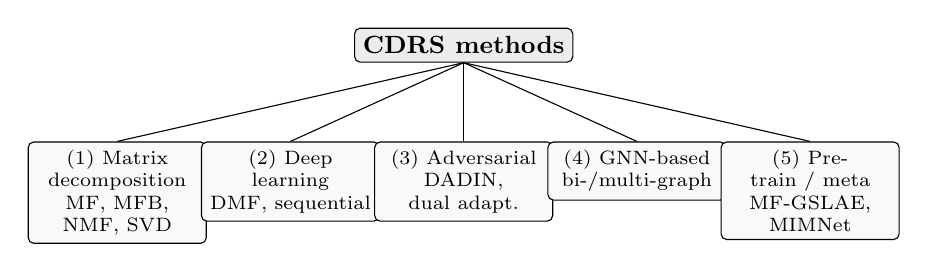
\begin{tikzpicture}[
  font=\scriptsize,
  box/.style={draw, rounded corners=2pt, align=center, inner sep=3pt},
  root/.style={box, fill=gray!15, font=\small\bfseries},
  leaf/.style={box, fill=gray!5, text width=2.05cm}
]
\node[root] (root) {CDRS methods};
\node[leaf, below=1.0cm of root, xshift=-4.4cm] (f1) {(1) Matrix decomposition\\MF, MFB, NMF, SVD};
\node[leaf, below=1.0cm of root, xshift=-2.2cm] (f2) {(2) Deep learning\\DMF, sequential};
\node[leaf, below=1.0cm of root] (f3) {(3) Adversarial\\DADIN, dual adapt.};
\node[leaf, below=1.0cm of root, xshift=2.2cm] (f4) {(4) GNN-based\\bi-/multi-graph};
\node[leaf, below=1.0cm of root, xshift=4.4cm] (f5) {(5) Pre-train / meta\\MF-GSLAE, MIMNet};
\foreach \n in {f1,f2,f3,f4,f5} {\draw (root.south) -- (\n.north);}
\end{tikzpicture}
\caption{Taxonomy of CDRS techniques used in this paper (five families).}
\label{fig:cdrs_taxonomy}
\end{figure}

\noindent\textbf{(1) Matrix decomposition-based.}
Low-rank factorization of rating matrices (MF, MFB, NMF, SVD)~\cite{koren2009matrix,lee2000algorithms,sarwar2002incremental}.
\textbf{(2) Deep learning-based.}
Non-linear or sequential neural recommenders~\cite{xue2017deep,he2017neural,ma2024triple,chen2025recurrent,wang2025hierarchical}.
\textbf{(3) Adversarial learning-based.}
Domain-adversarial alignment of feature distributions~\cite{li2022adversarial,kong2024dadin,su2024cross}.
\textbf{(4) Graph neural network-based.}
Transfer over user--item or multi-graph structures~\cite{zhao2025cross,gao2025disentangled}.
\textbf{(5) Pre-training / meta-learning-based.}
Multi-domain pre-training and meta-adaptation~\cite{wang2025mf,zhu2025mimnet}.
Table~\ref{tab:family_pros_cons} summarizes advantages and limitations of each family in the CDRS setting. This comparison motivates our focus on family~(1): complex CDRS models still rely on decomposition/embedding backbones whose controlled sparse-target behaviour remains under-compared.

\begin{table}[htbp]
\centering
\caption{Advantages and limitations of CDRS method families in cross-domain / sparse settings.}
\label{tab:family_pros_cons}
\renewcommand{\arraystretch}{1.2}
\small
\begin{tabular}{p{2.6cm} p{5.3cm} p{5.6cm}}
\toprule
\textbf{Family} & \textbf{Advantages} & \textbf{Limitations in CDRS / sparsity} \\
\midrule
Matrix decomposition & Interpretable factors; strong classical baselines; relatively efficient & May miss complex non-linearity; NMF non-negativity can restrict cross-domain alignment \\
Deep learning & Flexible non-linear / sequential modelling & Often data-hungry; harder to train fairly under extreme sparsity \\
Adversarial learning & Can reduce domain shift via distribution alignment & Adversarial training may be unstable when target ratings are scarce \\
Graph neural networks & Captures high-order user--item relations & Higher compute/memory cost; graph construction depends on available links \\
Pre-training / meta-learning & Reuses multi-domain signals; supports adaptation & Quality depends on pre-training data and overlap assumptions \\
\bottomrule
\end{tabular}
\end{table}

\begin{sidewaystable}[ht]
\centering
\caption{Summary of previous work on cross-domain recommendation.}
\label{tab:related_work_summary}
\renewcommand{\arraystretch}{1.25}
\setlength{\tabcolsep}{3pt}
\small
\begin{tabular}{l c p{2.2cm} p{2.6cm} p{2.0cm} p{3.2cm} p{3.8cm}}
\hline
\textbf{Reference} & \textbf{Year} & \textbf{Model / type} & \textbf{Datasets} & \textbf{Scenario} & \textbf{Reported performance} & \textbf{Focus}\\
\hline
Zang et al.~\cite{zang2022survey} & 2022 & Survey \& taxonomy & Multiple (review) & All & --- & CDRS overlap taxonomy (user/item/non-overlap). \\
Ayemowa et al.~\cite{ayemowa2024systematic} & 2024 & Survey (deep learning) & Multiple (review) & All & --- & Systematic review of deep learning in CDRS. \\
Patel \& Kant~\cite{patel2025enhanced} & 2025 & CF + transfer learning & Amazon category pairs & User overlap & MAE/RMSE on sparse targets & Classical CF with transfer for sparse targets. \\
Li et al.~\cite{li2022adversarial} & 2022 & Adversarial CDR & Cross-domain rating benchmarks & User overlap & MAE/RMSE (vs.\ CDR baselines) & Aligns user feature distributions across domains. \\
Kong et al.~\cite{kong2024dadin} & 2024 & DADIN & Amazon; Huawei & User overlap & AUC $+0.71\%$ (Amazon), $+0.08\%$ (Huawei) vs.\ strongest baseline & Domain-adversarial deep interest network. \\
Ma et al.~\cite{ma2024triple} & 2024 & Triple sequence learning & Cross-domain sequential benchmarks & User overlap & Ranking metrics (e.g., HR/NDCG) & Sequential behaviour of shared users. \\
Su et al.~\cite{su2024cross} & 2024 & Dual adversarial adaptation & Cross-domain benchmarks & Non-overlap & Ranking / accuracy vs.\ SOTA & Adversarial adaptation with limited overlap. \\
Wang et al.~\cite{wang2025mf} & 2025 & MF-GSLAE & Dual-target CDR benchmarks & User--item overlap & Ranking metrics vs.\ dual-target baselines & Multi-factor pre-training for dual-target CDR. \\
Zhao et al.~\cite{zhao2025cross} & 2025 & Adaptive bi-directional transfer GNN & Cross-domain graph benchmarks & User overlap & Ranking metrics vs.\ GNN/CDR baselines & Bi-directional graph transfer. \\
Gao et al.~\cite{gao2025disentangled} & 2025 & Disentangled multi-graph convolution & Multi-domain interaction graphs & User / item overlap & Ranking metrics vs.\ graph CDR baselines & Disentangled multi-graph domain correlation. \\
\hline
\end{tabular}
\end{sidewaystable}

As indicated in Table \ref{tab:related_work_summary}, the vast majority of recent highly impactful studies focus primarily on the development of complex deep learning or graph neural network architectures. While complex architectures are certainly effective, their increasing complexity makes it difficult to assess the impact of the underlying decomposition method. It is striking that there has been little to no systematic comparison of fundamental decomposition methods under controlled conditions with varying levels of sparsity to determine which will provide the best baseline for knowledge transfer performance. This study addresses this deficit by providing a rigorous comparison of MF, MFB, NMF, DMF, and SVD in order to identify a clear baseline for knowledge transfer performance and thereby clarify the inherent value of fundamental approaches.

A related risk in CDRS is \emph{negative transfer}, where source-domain knowledge harms target performance~\cite{zhang2021transferability,wang2019characterizing}. Our later experiments show this risk concretely for NMF\_CDRS, where the non-negativity constraint appears to impede flexible latent-space alignment across domains.




\section{Methodological Framework}
The purpose of this section is to provide a solution for the problem of data sparseness as defined at the beginning of this section by presenting a mathematical representation of the problem and describing five different decomposition approaches that can be used to transfer knowledge between the source domain ($R^S$) and the target domain ($R^T$), which share users.


\subsection{Notations and Preliminaries}
To help understand our framework, we list the main mathematical notations used in this paper in Table \ref{tab:notations}.

\begin{table}[ht]
\centering
\caption{Summary of Key Notations}
\label{tab:notations}
\renewcommand{\arraystretch}{1.2}
\begin{tabular}{l p{10cm}}
\toprule
\textbf{Symbol} & \textbf{Description} \\
\midrule
$U, I$ & Sets of users and items, respectively \\
$n, m$ & Number of users ($|U|$) and items ($|I|$) \\
$R^S, R^T$ & Rating matrices for Source ($S$) and Target ($T$) domains \\
$r_{ui}, \hat{r}_{ui}$ & Observed and predicted rating for user $u$ on item $i$ \\
$P, Q$ & Latent factor matrices for users ($n \times d$) and items ($m \times d$) \\
$d$ & Dimension of the latent factor space \\
$C_U, C_I$ & Sets of common users ($U^S \cap U^T$) and common items ($I^S \cap I^T$) \\
$b_u, b_i$ & Bias terms for user $u$ and item $i$ \\
$\mu$ & Global average rating \\
$\lambda$ & Regularization hyperparameter to prevent overfitting \\
$\gamma$ & Transfer trade-off parameter controlling knowledge alignment \\
$\eta$ & Learning rate for Stochastic Gradient Descent (SGD) \\
$\mathcal{L}$ & Objective function (Loss) to be minimized \\
\bottomrule
\end{tabular}
\end{table}

\subsection{Problem Formulation}
Let the set of users be denoted by $U$, with its size being $n=|U|$. The items are partitioned into two distinct domains: a source domain with an item set $I^S$ of size $m_S=|I^S|$, and a target domain with an item set $I^T$ of size $m_T=|I^T|$.

The user-item interactions within these domains are captured by two corresponding rating matrices, $R^S \in \mathbb{R}^{n \times m_S}$ and $R^T \in \mathbb{R}^{n \times m_T}$, where an entry $r_{u,i}$ represents the observed rating given by user $u \in U$ to an item $i$.The extent of possible transferable knowledge between different domains depends upon how much their respective users and items have in common. There are four possible types of relationships between two domains that we can identify as shown in Figure \ref{fig:overlap}.



\begin{figure}[htbp]
    \centering
    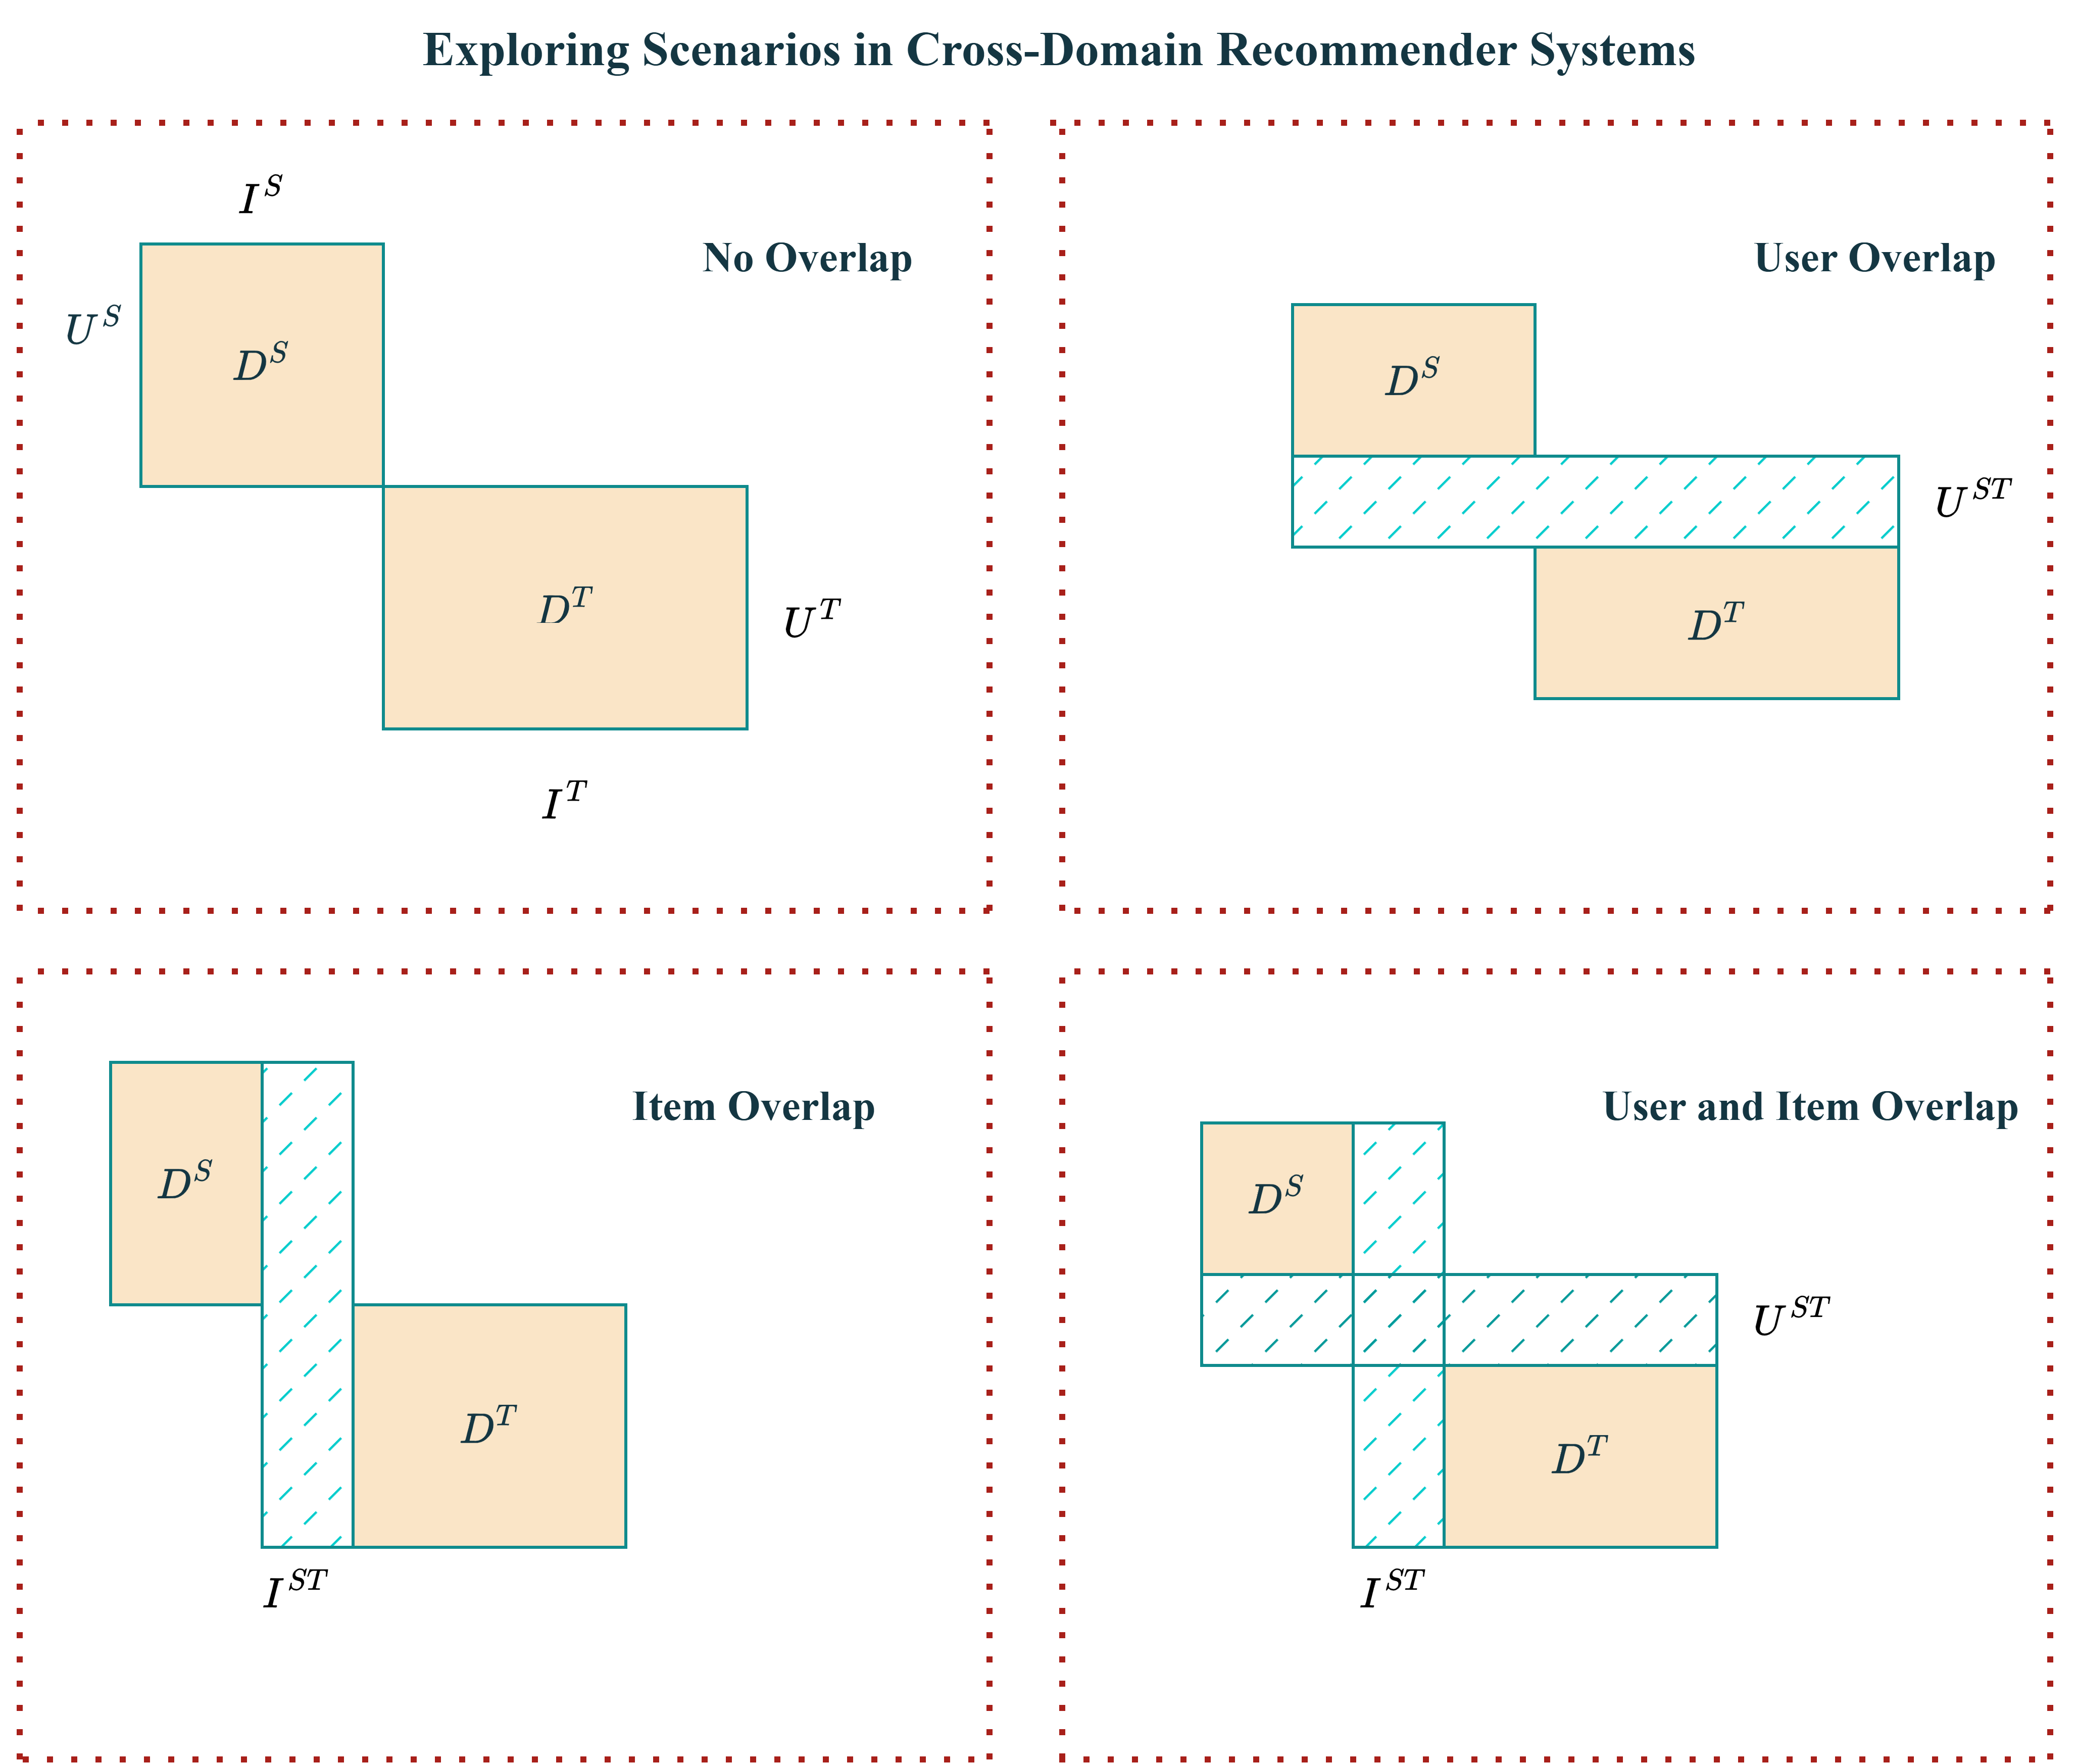
\includegraphics[width=0.8\textwidth]{Fig.1.png} % Adjust the path
    \caption{Overlap Scenarios in Cross-domain recommendation system}
    \label{fig:overlap}
\end{figure}





\begin{enumerate}
    \item \textbf{User Overlap:} A subset of users is shared across domains, while the item sets are disjoint ($U^S \cap U^T \neq \emptyset$ and $I^S \cap I^T = \emptyset$).
    \item \textbf{Item Overlap:} A subset of items is shared, but the user populations are distinct ($U^S \cap U^T = \emptyset$ and $I^S \cap I^T \neq \emptyset$).
    \item \textbf{User and Item Overlap:} Both the user and item sets have a non-empty intersection ($U^S \cap U^T \neq \emptyset$ and $I^S \cap I^T \neq \emptyset$).
    \item \textbf{No Overlap (Disjoint):} The user and item sets are entirely separate ($U^S \cap U^T = \emptyset$ and $I^S \cap I^T = \emptyset$).
\end{enumerate}



The user overlap and item overlap are of particular interest due to the fact that they are the most common types of relationships found in many real world applications where users interact with multiple catalogs of items (books/movies; e-commerce/finance) etc. However, in both of these cases there exists a significant problem resulting from the lack of data in the target domain. Specifically, we measure the severity of this issue through the density metric:

\begin{equation}
\mathrm{density}(R) = \frac{|\{(u,i): r_{u,i} \mathrm{\ is\ observed} \}|}{|U| \times |I|}
\end{equation}

where the target domain's density is significantly lower than the source domain's, i.e., $\mathrm{density}(R^T) \ll \mathrm{density}(R^S)$. This condition makes learning a reliable model from $R^T$ alone an ill-posed problem, leading to poor generalization and compounding the cold-start problem.

Formally, the problem studied in this paper is as follows. \emph{(i) Measurable failure modes:} under high target sparsity, classical decompositions can fail in distinct ways---for example, non-negativity-constrained transfer (NMF) and shallow non-linear interaction transfer (DMF) may yield substantially higher MAE/RMSE than bias-aware factorization, as quantified later under matched protocols. \emph{(ii) Why complex architectures alone do not resolve this gap:} sophisticated CDRS models still rely on an underlying decomposition or embedding backbone; without a controlled comparison of those backbones under fixed sparsity, it remains unclear whether gains come from the backbone or from the surrounding architecture. \emph{(iii) Scope of this work:} we restrict attention to the \textbf{user-overlap} scenario ($U^S \cap U^T \neq \emptyset$, $I^S \cap I^T = \emptyset$), adapt five foundational decompositions (MF, MFB, NMF, SVD, DMF) to a two-phase source-to-target transfer setting, and compare them under identical hyperparameters and training-set sizes (20\%--80\%) using MAE and RMSE. Item-overlap and no-overlap settings, and new complex architectures, are outside the present scope.

\subsection{Decomposition Approaches}

\subsubsection{Matrix Factorization for Cross-Domain Recommendation (MF\_CDRS)}

At the core of our approach is the standard matrix factorization. We are seeking to represent the user-item rating matrix $R$ as the product of two latent factor matrices of lower rank: a user latent matrix $P$ and an item latent matrix $Q$. The predicted rating $\hat{r}_{ui}$ of a given user $u$, and item $i$, will be the dot-product of their respective latent factors:


\begin{equation}
\hat{r}_{ui} = P_u^T Q_i
\end{equation}


To determine these factors, we first train the source-domain factorization with the following regularized squared error objective ($P^S, Q^S$):

\begin{equation}
\mathcal{L}_{Source} = \sum_{(u,i) \in R^S} (r_{ui} - (P_u^S)^T Q_i^S)^2 + \lambda(\|P_u^S\|^2 + \|Q_i^S\|^2)
\end{equation}


Here, $R^S$ is the set of known ratings in the source domain, and $\lambda$ is the L2 regularization hyperparameter to prevent overfitting to this data. We then use the learned factors $P^S$ and $Q^S$ from training on the source domain as a starting point to train the model on the target domain.

% Figure 2 Placeholder
\begin{figure}[ht]
    \centering
    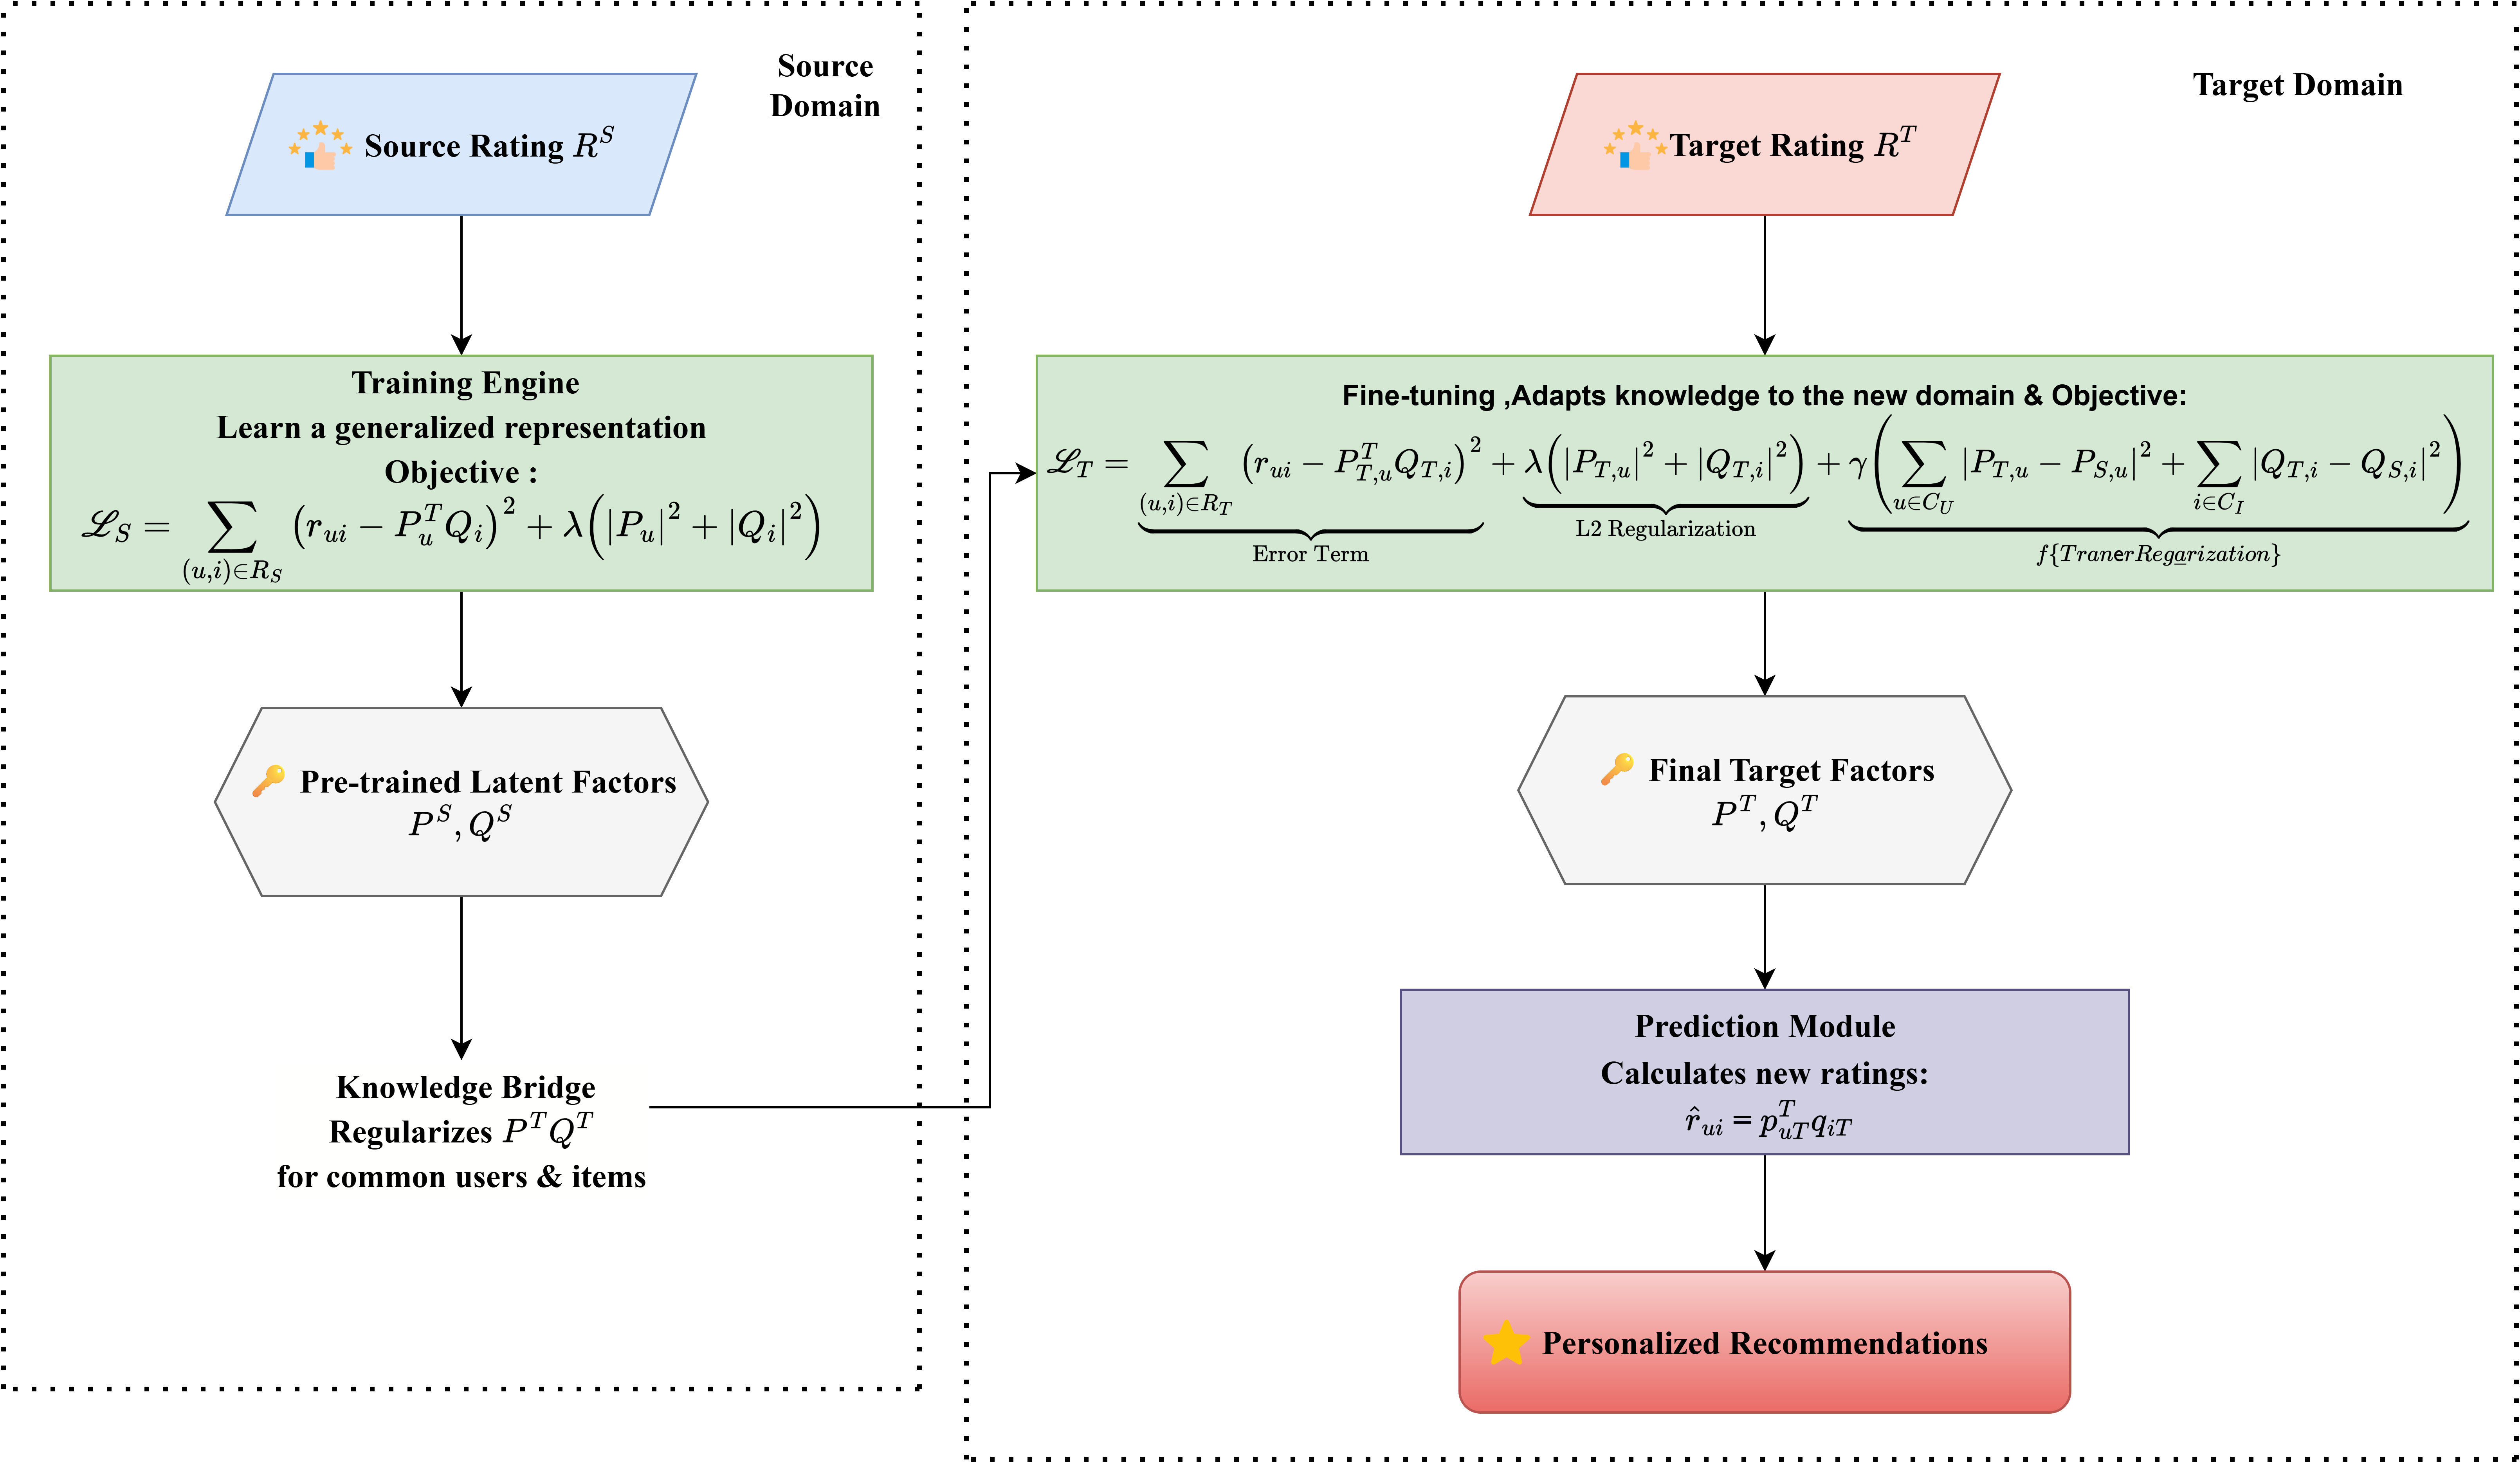
\includegraphics[width=0.8\textwidth]{Fig. 2.png} % Uncomment and add image path
    \caption{Framework of the Matrix Factorization (MF) adaptation used in this comparative study.}
    \label{fig:mf_cdrs}
\end{figure}



The overall model structure, as shown in Figure \ref{fig:mf_cdrs}, illustrates how the two stages (the source training stage and the target training stage) are connected. In order to allow for the transfer of knowledge between these two domains, we introduce an additional term into our loss function that forces the latent features of common users and items to be consistent across both domains. The full objective function for learning the target domain factors ($P^T, Q^T$) is:



\begin{equation}
\begin{aligned}
\mathcal{L}_{Target} = \sum_{(u,i) \in R^T} (r_{ui} - (P_u^T)^T Q_i^T)^2 + \lambda \sum_{(u,i) \in R^T} (\|P_u^T\|^2 + \|Q_i^T\|^2) \\
+ \gamma \left( \sum_{u \in C_U} \|P_u^T - P_u^S\|^2 + \sum_{i \in C_I} \|Q_i^T - Q_i^S\|^2 \right)
\end{aligned}
\end{equation}



Here, we denote by $R^T$ the set of known ratings in the target domain, by $C_U$ is the set of common users in both domains, $C_I$ is the set of common items between domains, and $\gamma$ is a hyperparameter that is used to control how much the model will learn from one domain and apply it to the other. We also use Stochastic Gradient Descent (SGD) to find the optimal parameters for the model by minimizing the target objective function. The SGD update rules are:




\begin{equation}
P_u^T \leftarrow P_u^T + \eta \left( (r_{ui} - \hat{r}_{ui})Q_i^T - \lambda P_u^T - \gamma (P_u^T - P_u^S) \right)
\end{equation}

\begin{equation}
Q_i^T \leftarrow Q_i^T + \eta \left( (r_{ui} - \hat{r}_{ui})P_u^T - \lambda Q_i^T - \gamma (Q_i^T - Q_i^S) \right)
\end{equation}



Here, $\eta$ is the learning rate; for a non-common user or item, the final term of $\gamma$  is dropped.


\subsubsection{Matrix Factorization with Bias for Cross-Domain Recommendation (MFB\_CDRS)}

The addition of the bias term in this approach improves the original matrix factorization model with the inclusion of baseline rating characteristics: user-specific bias ($b_u$), item-specific bias ($b_i$), and global average rating ($\mu$). This extends the rating prediction function for an individual rating $\hat{r}_{ui}$ as follows:



\begin{equation}
\hat{r}_{ui} = \mu + b_u + b_i + P_u^T Q_i
\end{equation}

First, we train the model on the source domain by minimizing a regularized squared error objective function, $\mathcal{L}_{Source}$, which includes all latent factors and bias terms:

\begin{equation}
\mathcal{L}_{Source} = \sum_{(u,i) \in R^S} (r_{ui} - \hat{r}_{ui}^S)^2 + \lambda \left( \|P_u^S\|^2 + \|Q_i^S\|^2 + (b_u^S)^2 + (b_i^S)^2 \right)
\end{equation}

For the target domain, we apply Transfer Regularization. The objective function $\mathcal{L}_{Target}$ includes an additional penalty that minimizes the divergence of the target domain parameters from the pre-trained source parameters for all common entities.

\begin{equation}
\begin{aligned}
\mathcal{L}_{Target} = \sum_{(u,i) \in R^T} (r_{ui} - \hat{r}_{ui}^T)^2 + \lambda \sum_{(u,i) \in R^T} (\|P_u^T\|^2 + \|Q_i^T\|^2 + (b_u^T)^2 + (b_i^T)^2) \\
+ \gamma \left( \sum_{u \in C_U} (\|P_u^T - P_u^S\|^2 + (b_u^T - b_u^S)^2) + \sum_{i \in C_I} (\|Q_i^T - Q_i^S\|^2 + (b_i^T - b_i^S)^2) \right)
\end{aligned}
\end{equation}

We optimize the model using Stochastic Gradient Descent (SGD). After calculating the error $e_{ui} = r_{ui} - \hat{r}_{ui}$, we update the target domain parameters. For common entities, the update rules are:

\begin{equation}
P_u^T \leftarrow P_u^T + \eta \left( e_{ui} Q_i^T - \lambda P_u^T - \gamma (P_u^T - P_u^S) \right)
\end{equation}

\begin{equation}
Q_i^T \leftarrow Q_i^T + \eta \left( e_{ui} P_u^T - \lambda Q_i^T - \gamma (Q_i^T - Q_i^S) \right)
\end{equation}

\begin{equation}
b_u^T \leftarrow b_u^T + \eta \left( e_{ui} - \lambda b_u^T - \gamma (b_u^T - b_u^S) \right)
\end{equation}

\begin{equation}
b_i^T \leftarrow b_i^T + \eta \left( e_{ui} - \lambda b_i^T - \gamma (b_i^T - b_i^S) \right)
\end{equation}

For entities not present in the source domain, the final transfer regularization term (the term multiplied by $\gamma$) in each rule is dropped.

\subsubsection{Non-negative Matrix Factorization for Cross-Domain Recommendation (NMF\_CDRS)}



This approach uses an adaptation of Non-negative Matrix Factorization (NMF) for a cross-domain recommendation task. As indicated in \textbf{Fig. \ref{fig:nmf_cdrs}}, the primary architecture of this framework is a two-phase process; first, latent factors are learned from a dense source domain, and these learned latent factors are then used as guidance during the learning of a sparse target domain. NMF's non-negativity constraint helps ensure that learned factors are more understandable.




% Figure 3 Placeholder
\begin{figure}[ht]
    \centering
    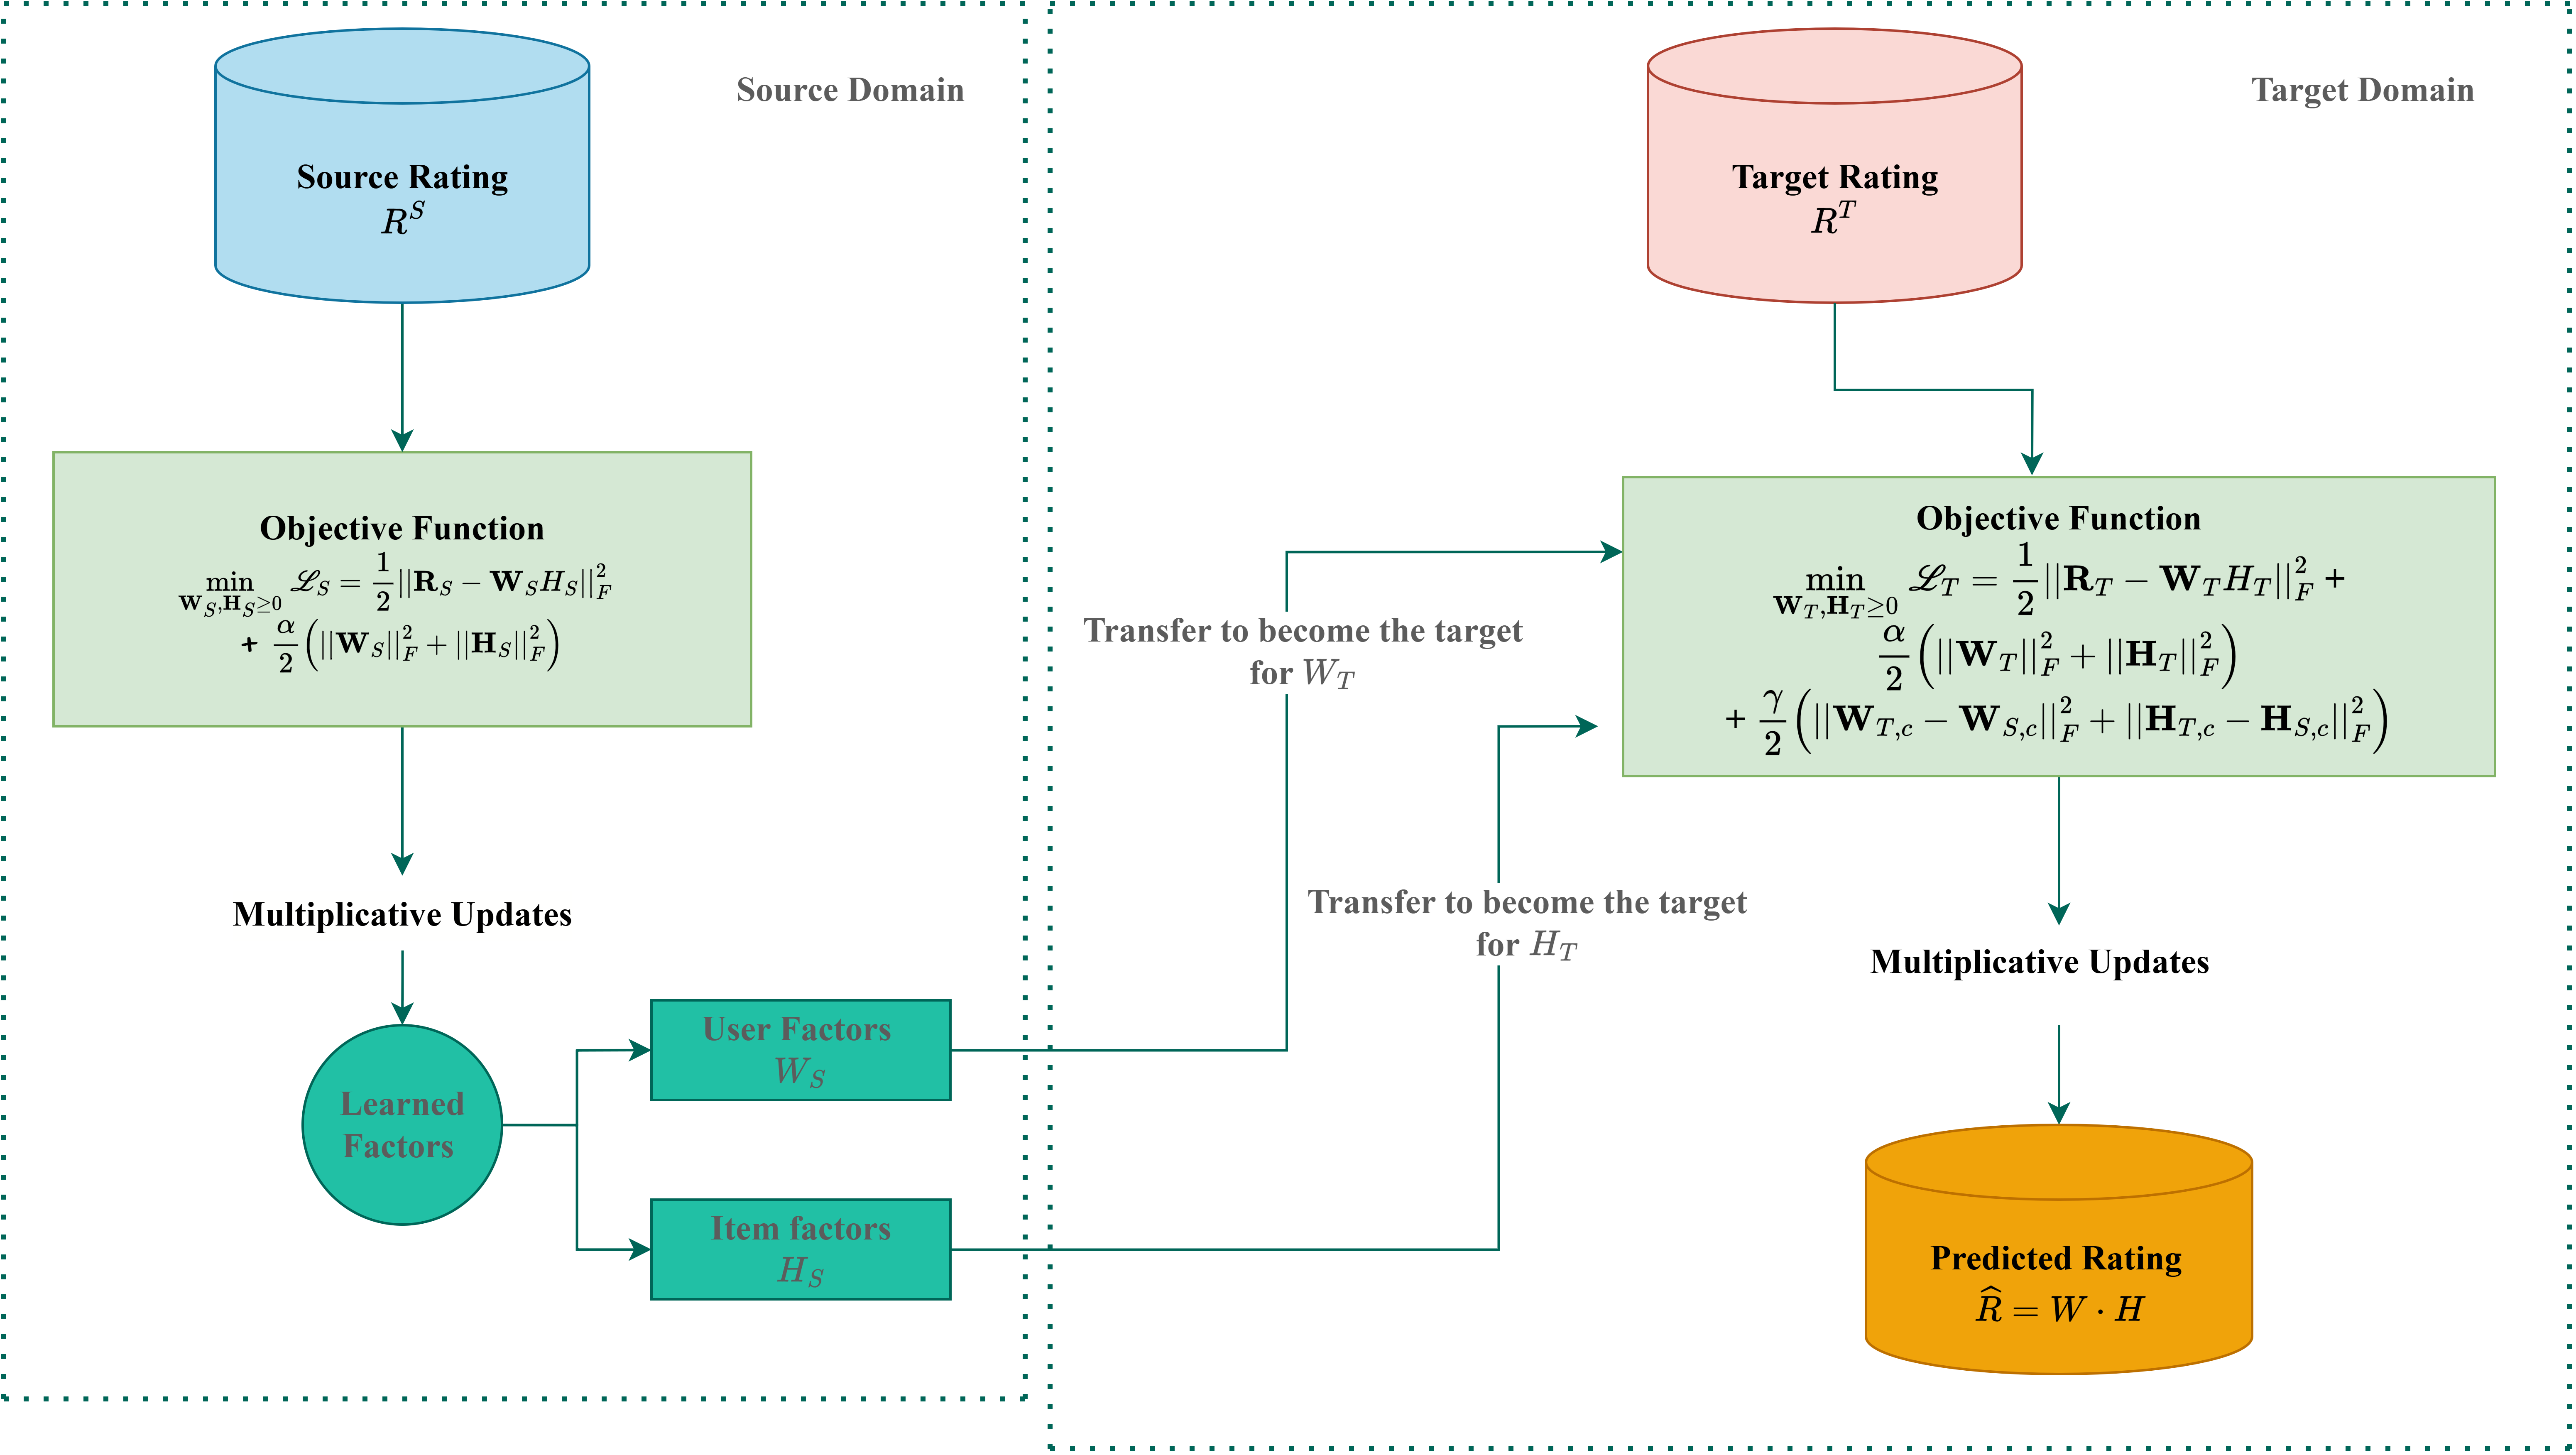
\includegraphics[width=0.8\textwidth]{Fig.3.png} % Uncomment and add image path
    \caption{Framework of the Non-negative Matrix Factorization (NMF) adaptation used in this comparative study.}
    \label{fig:nmf_cdrs}
\end{figure}

The initial phase involves training a regularized NMF model on the source domain rating matrix, $R^S$. The objective is to decompose $R^S$ into two non-negative latent factor matrices: a user-factor matrix $W^S \in \mathbb{R}^{n \times d}$ and an item-factor matrix $H^S \in \mathbb{R}^{m_S \times d}$. The objective function to be minimized is:

\begin{equation}
\min_{W^S, H^S \geq 0} \mathcal{L}_S = \frac{1}{2} \|R^S - W^S (H^S)^T\|_F^2 + \frac{\alpha}{2} (\|W^S\|_F^2 + \|H^S\|_F^2)
\end{equation}

where $\alpha$ is the regularization hyperparameter and $\|\cdot\|_F^2$ denotes the squared Frobenius norm.



During the second phase, the knowledge gathered in the pre-trained source latent factors ($W^S, H^S$) will be used to guide the training of the target domain model. This is done with an added transfer regularizer as part of the target domain's objective function. It computes the penalty for the target factors ($W^T$, $H^T$) being far from the source variable for each user and item found in both domains. The total objective function for the target domain is:

\begin{equation}
\begin{aligned}
\min_{W^T, H^T \geq 0} \mathcal{L}_T = \frac{1}{2} \|R^T - W^T (H^T)^T\|_F^2 + \frac{\alpha}{2} (\|W^T\|_F^2 + \|H^T\|_F^2) \\
+ \frac{\gamma}{2} (\|W_c^T - W_c^S\|_F^2 + \|H_c^T - H_c^S\|_F^2)
\end{aligned}
\end{equation}

Here, the subscript $c$ indicates the factors corresponding to common entities. The hyperparameter $\gamma$ controls the influence of the transfer term. This objective is also optimized using modified multiplicative update rules derived from the gradients of $\mathcal{L}^T$:

\begin{equation}
W^T \leftarrow W^T \odot \frac{R^T H^T + \gamma W_c^S}{W^T (H^T)^T H^T + \alpha W^T + \gamma W_c^T}
\end{equation}

\begin{equation}
H^T \leftarrow H^T \odot \frac{(R^T)^T W^T + \gamma H_c^S}{H^T (W^T)^T W^T + \alpha H^T + \gamma H_c^T}
\end{equation}


Here, $\odot$ denotes element-wise multiplication, and the division is also element-wise. Note that the $\gamma$ terms in the update rules are only applied to the rows/columns corresponding to common entities; for non-common entities, these terms are zero.


\subsubsection{Singular Value Decomposition for Cross-Domain Recommendation (SVD\_CDRS)}



This approach is diagrammatically depicted in Figure \ref{fig:svd_cdrs} and consists of a two-phase procedure to obtain knowledge of a dense source domain and to apply it to a sparse target domain.

% Figure 4 Placeholder
\begin{figure}[ht]
    \centering
    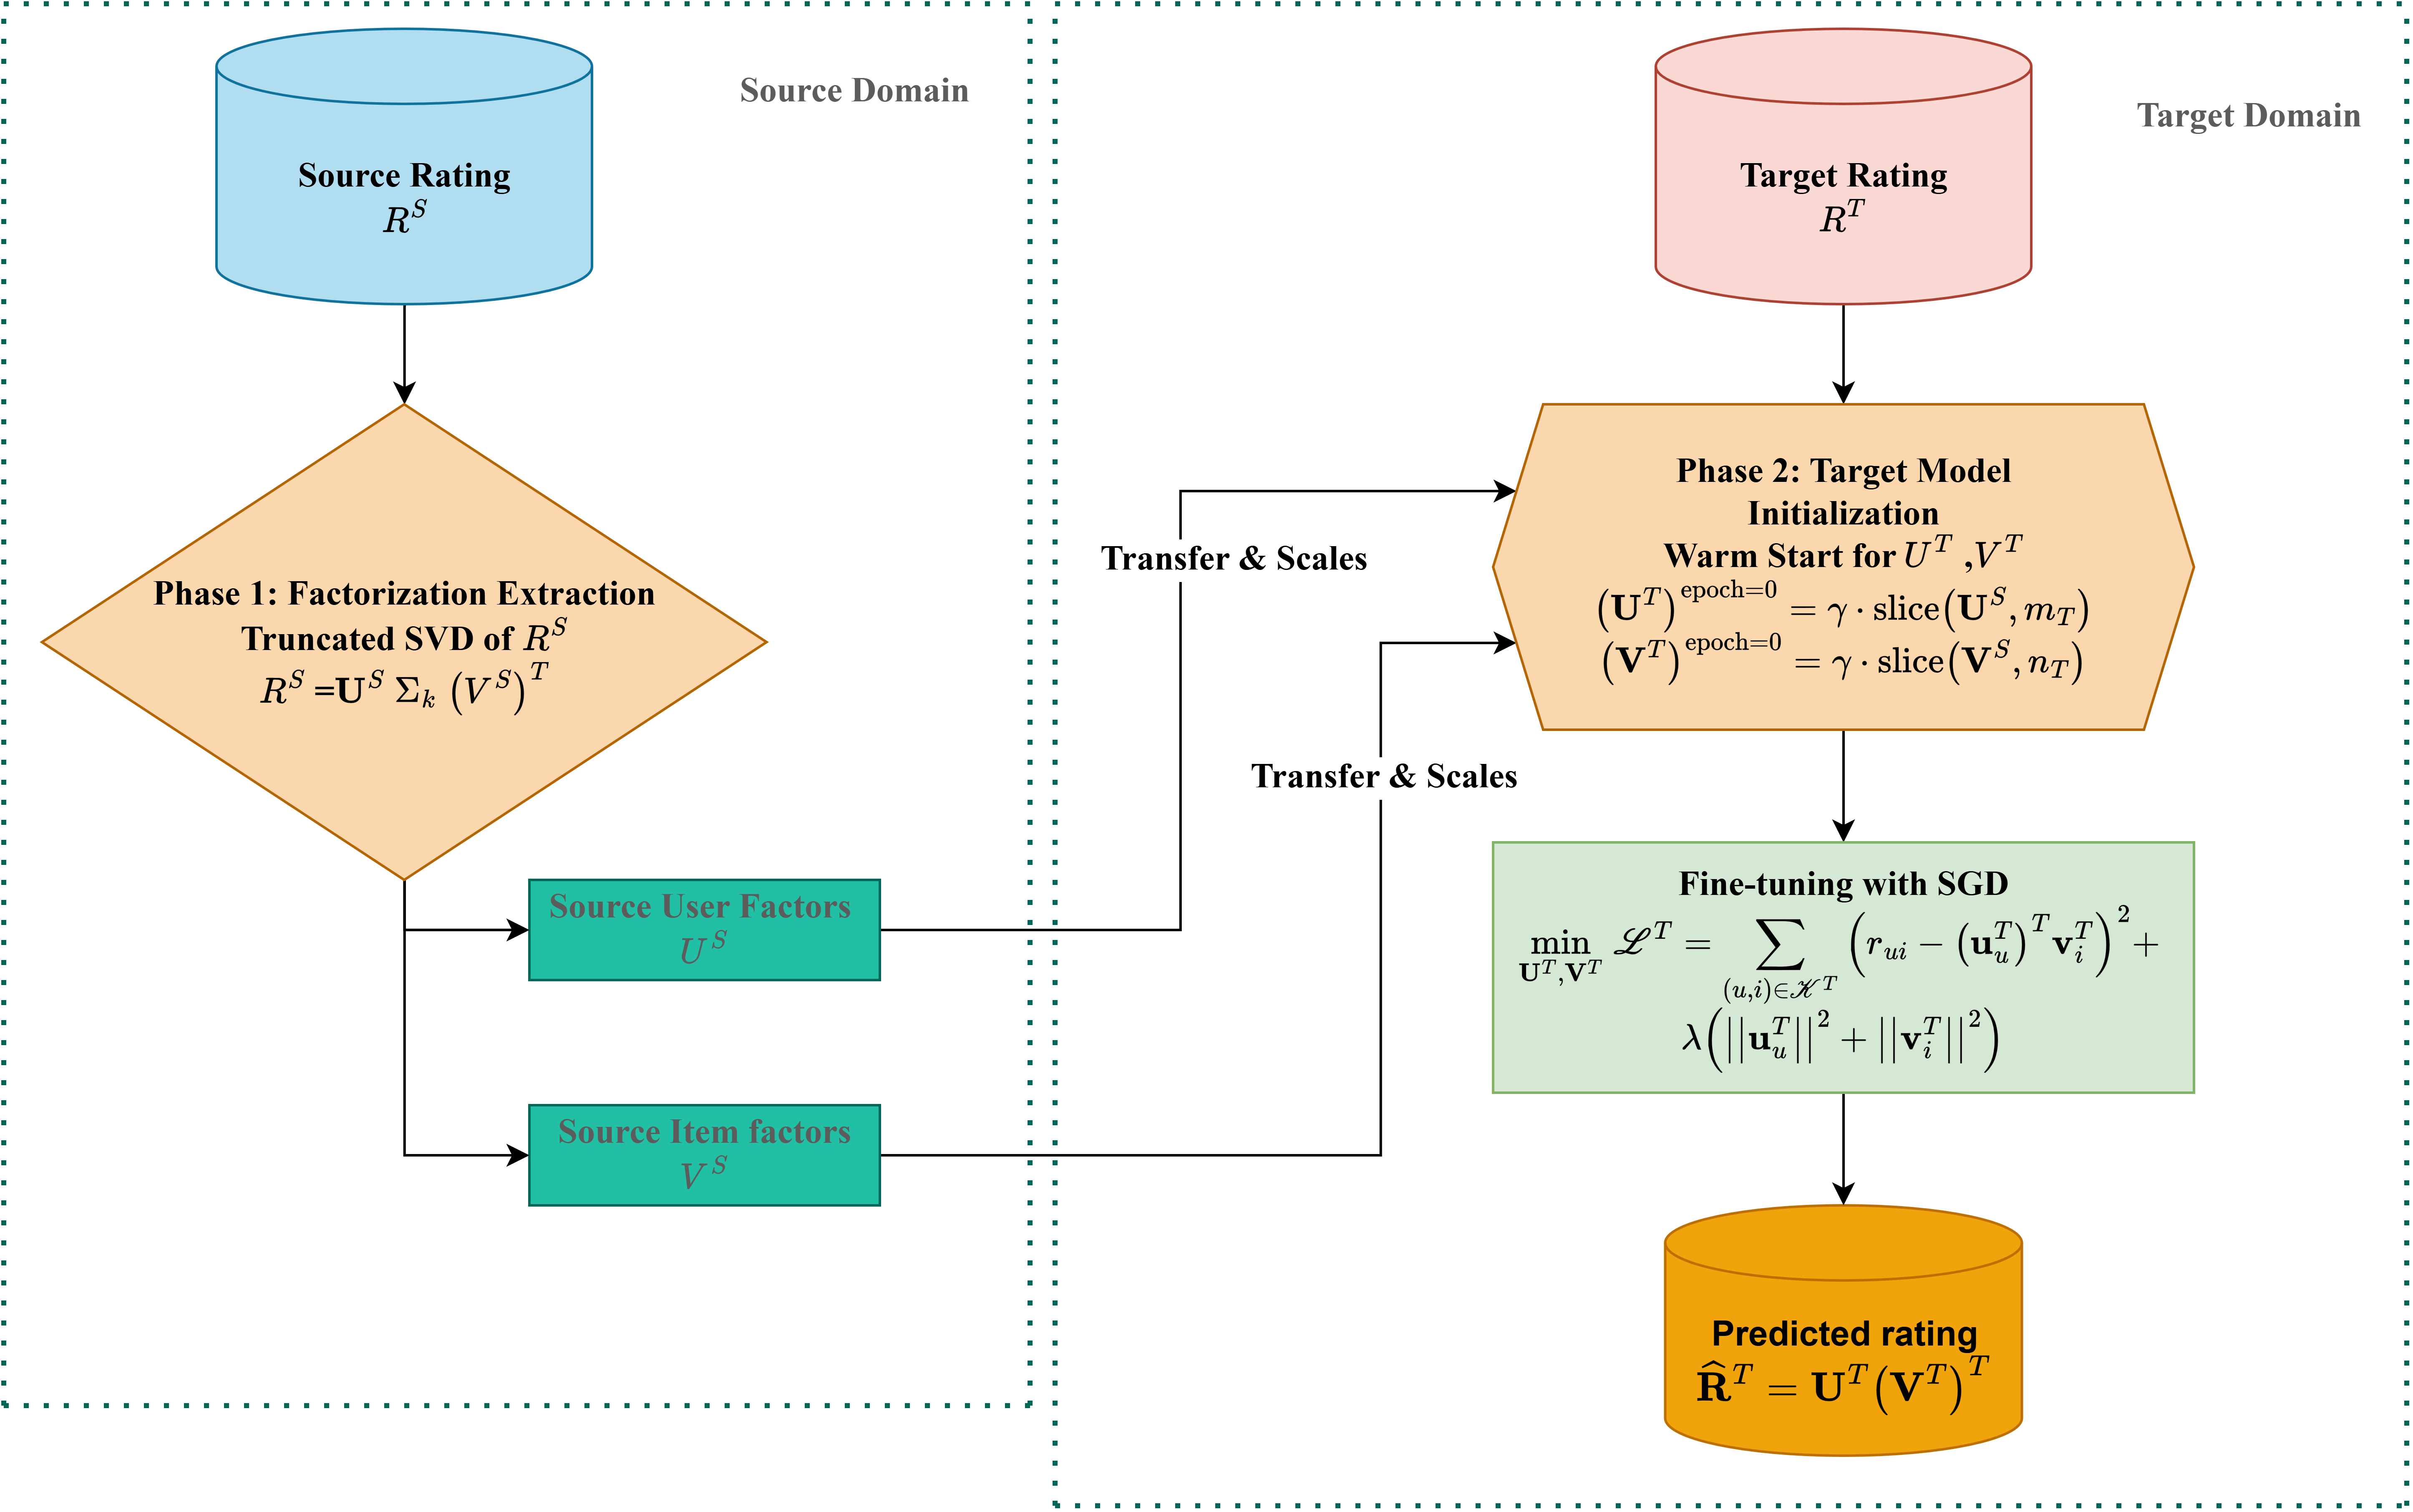
\includegraphics[width=0.8\textwidth]{Fig 4..png} % Uncomment and add image path
    \caption{Framework of the Singular Value Decomposition (SVD) adaptation used in this comparative study.}
    \label{fig:svd_cdrs}
\end{figure}



First, we will obtain reliable latent factors of the source domain by means of a fixed decomposition technique, namely, Singular Value Decomposition (SVD). Then we will use this as an appropriate starting point to refine the model with the subsequent target domain data.

Firstly, we determine the quality of the latent variables of the dense source rating matrix, $R^S$. Therefore, we find the optimal low-rank representation of the source matrix by applying SVD. We obtain the truncated SVD of $R^S$ by:


\begin{equation}
R^S \approx U^S \Sigma (V^S)^T
\end{equation}

where $U^S \in \mathbb{R}^{n \times d}$ and $V^S \in \mathbb{R}^{m_S \times d}$ are the matrices containing the latent factors for source users and items, respectively, and $d$ is the number of latent dimensions.



The second phase consists of training a model for the target domain. A major contribution of this approach is how it initializes $U^T$ and $V^T$, the latent factor matrices for the target domain; as opposed to randomizing the values, we initialize the factors for shared entities directly from the pre-computed source factors:

\begin{equation}
U_c^T(initial) \leftarrow \gamma \cdot U_c^S
\end{equation}

\begin{equation}
V_c^T(initial) \leftarrow \gamma \cdot V_c^S
\end{equation}

After this "warm start" initialization, the target factors are fine-tuned by training on the available ratings in the sparse target matrix, $R^T$. The training is performed using Stochastic Gradient Descent (SGD) to minimize the standard regularized squared error objective function:

\begin{equation}
\min_{U^T, V^T} \mathcal{L}_T = \sum_{(u,i) \in R^T} (r_{ui} - (U_u^T)^T V_i^T)^2 + \lambda (\|U_u^T\|^2 + \|V_i^T\|^2)
\end{equation}

where $U_u^T$ and $V_i^T$ are the latent factor vectors for user $u$ and item $i$ in the target domain, and $\lambda$ is the regularization parameter.



\subsubsection{Deep Matrix Factorization for Cross-Domain Recommendation (DMF\_CDRS)}

Deep Matrix Factorization for recommendation is commonly associated with Xue et al.~\cite{xue2017deep}. The interaction used here---an element-wise (Hadamard) product of user and item latent factors followed by a weighted linear layer---is closer to the Generalized Matrix Factorization (GMF) component of Neural Collaborative Filtering~\cite{he2017neural} than to a deep multi-layer tower; we therefore treat DMF\_CDRS as a shallow non-linear interaction baseline rather than a full deep recommender. Concretely, there is no deeper MLP beyond that single linear layer, no non-linear activation on the prediction head, and no dropout or batch normalization; regularization is the same $\lambda$ weight decay used for the other methods (Figure~\ref{fig:dmf_cdrs}).

As depicted in Figure \textbf{\ref{fig:dmf_cdrs}}, the key concept does not involve transferring the latent space representations of the users and items, but rather the interaction function learned by the model. The interaction function models how user and item latent space representations are combined to create a rating.

% Figure 5 Placeholder
\begin{figure}[ht]
    \centering
    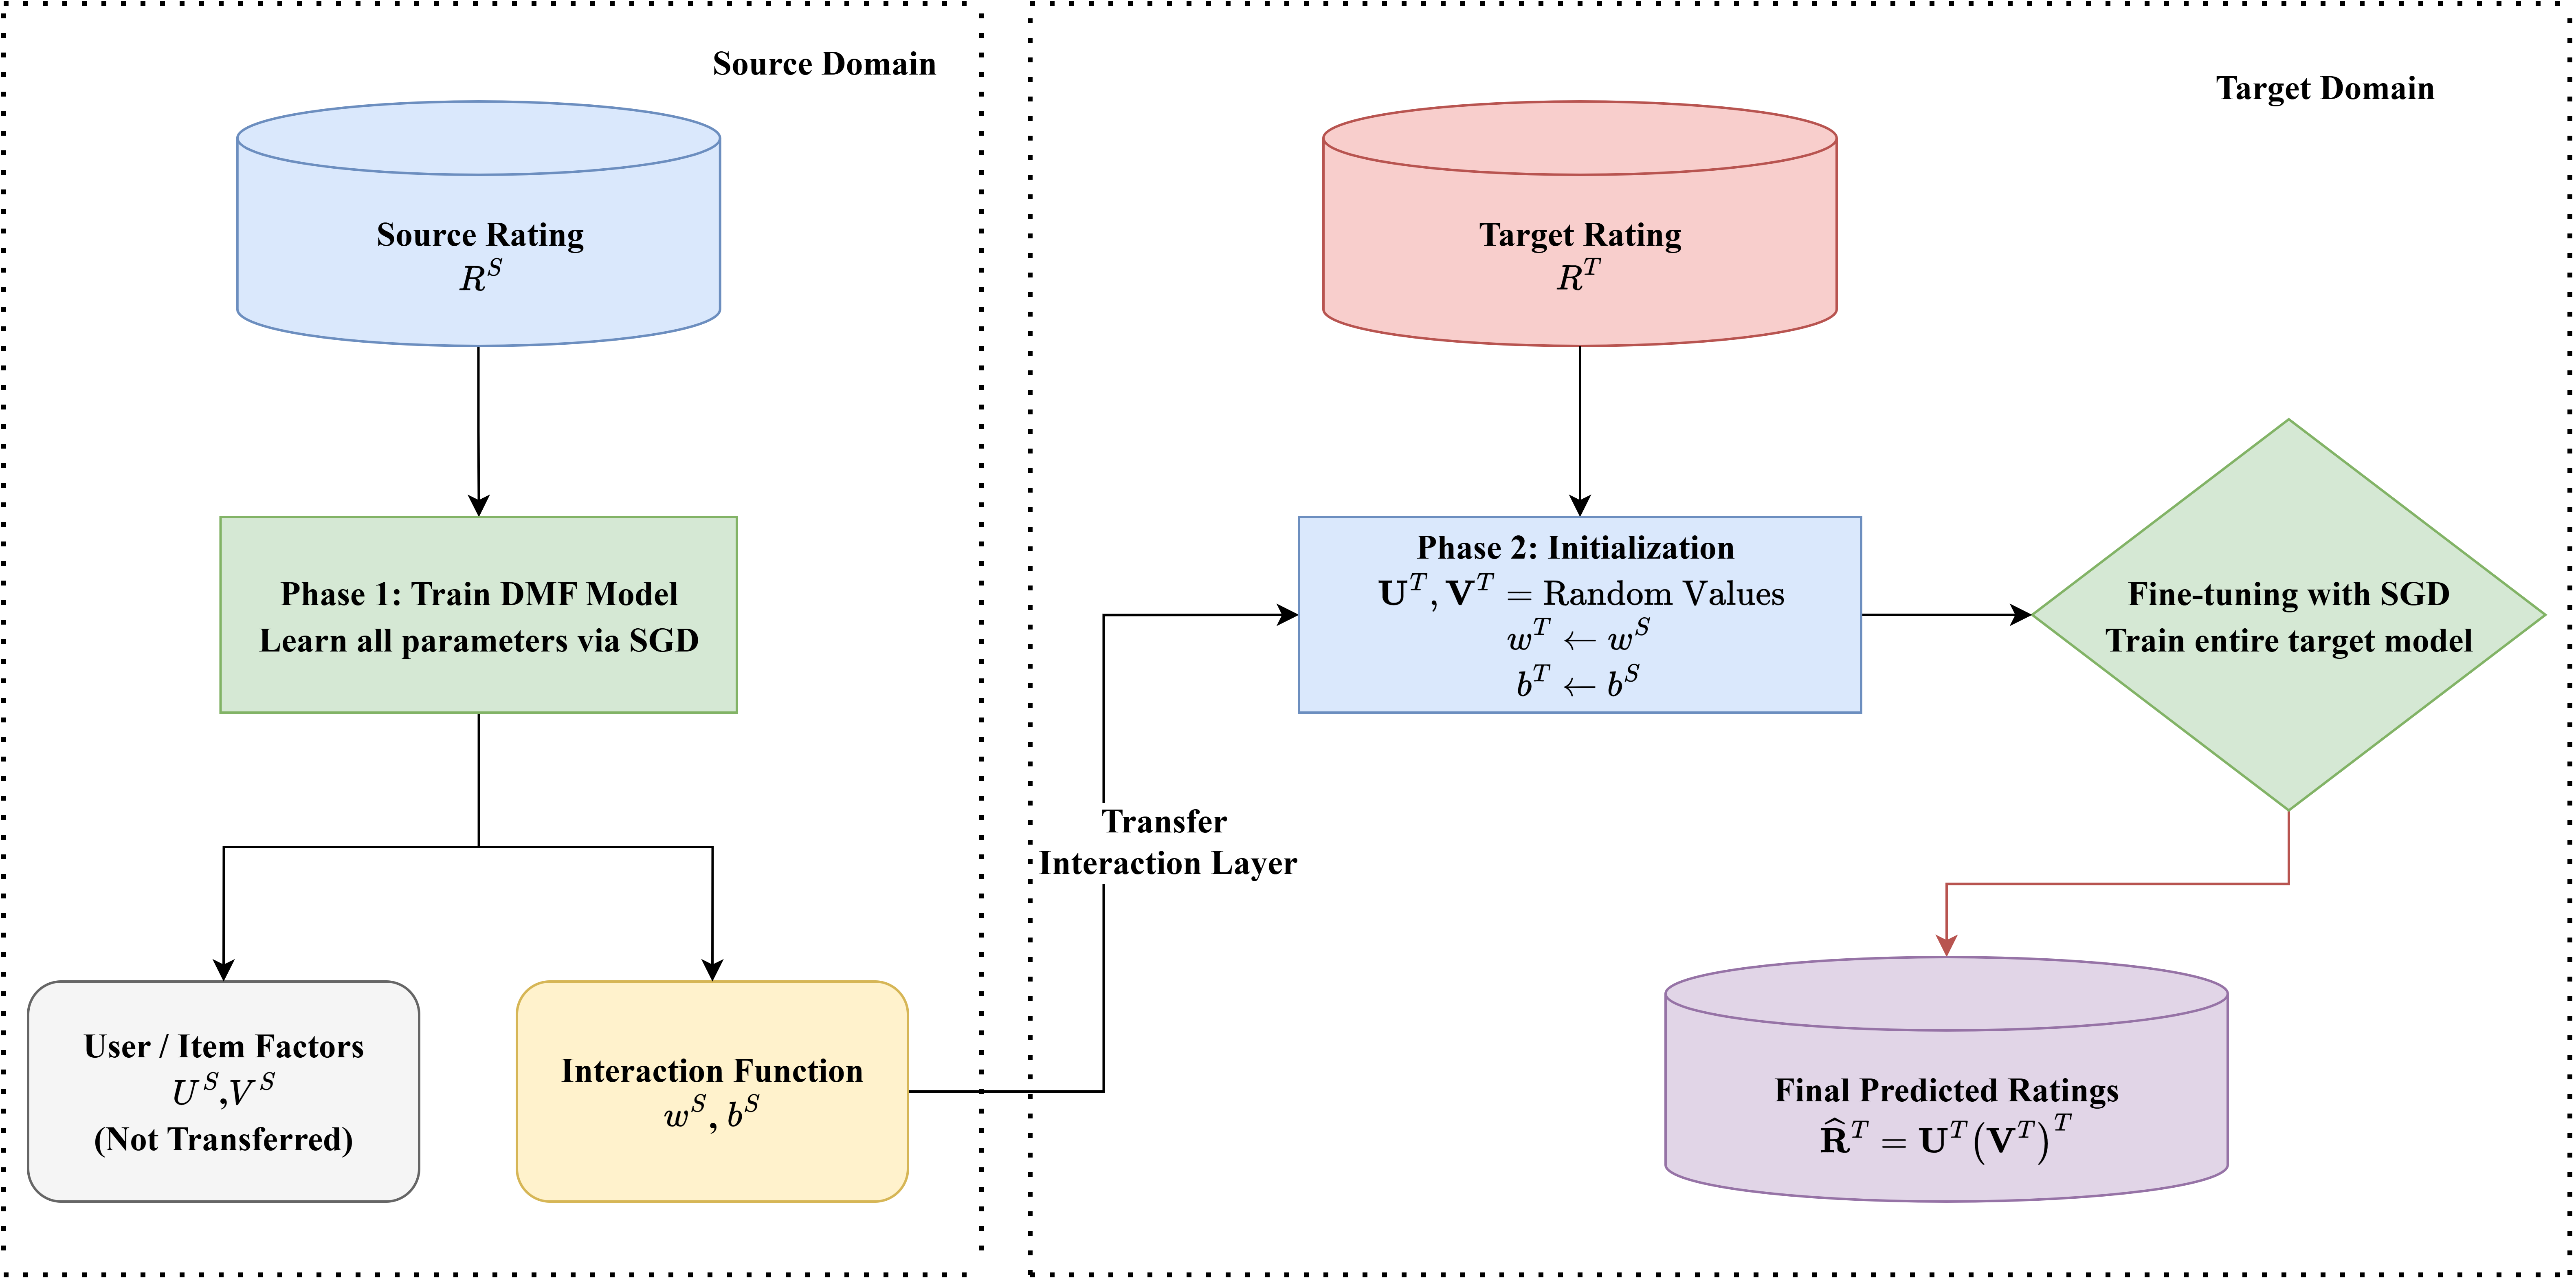
\includegraphics[width=0.8\textwidth]{Fig.5.png} % Uncomment and add image path
    \caption{Framework of the Deep Matrix Factorization (DMF) adaptation used in this comparative study.}
    \label{fig:dmf_cdrs}
\end{figure}


First, the model creates a latent representation for each user, denoted as $u$, and each item, denoted as $i$. Rather than using a simple dot product to compute the interaction between the latent space representations of the user and the item ($U_u$), the interaction is computed using a two-phase process: First, an element-wise product (Hadamard product, $\odot$) is applied to the latent space representations of the user and the item ($z_{ui} = U_u \odot V_i$). Second, the output from the first phase ($z_{ui}$) is passed through a final linear layer to generate the predicted rating using weights $w$ and a bias term $b$.

\begin{equation}
\hat{r}_{ui} = w^T (U_u \odot V_i) + b
\end{equation}

In the first phase, a complete DMF model is trained on the dense source domain matrix, $R^S$. This involves learning the source user factors ($U^S$), source item factors ($V^S$), and, most importantly, the parameters of the interaction function ($w^S$ and $b^S$). The model is trained by minimizing a regularized squared error objective function:

\begin{equation}
\min_{U^S, V^S, w^S, b^S} \mathcal{L}_S = \sum_{(u,i) \in R^S} (r_{ui} - \hat{r}_{ui}^S)^2 + \lambda (\|U^S\|_F^2 + \|V^S\|_F^2 + \|w^S\|^2 + (b^S)^2)
\end{equation}

During the second phase of training, we construct a new DMF model for our target domain. It is in this second phase that we perform the knowledge transfer. We take the parameters of the interaction function (i.e., $w^S$, $b^S$), which were previously learned during the first phase as part of the source domain, and copy them into the interaction function of our target model to serve as an initialization.

\begin{equation}
w^T \leftarrow w^S
\end{equation}

\begin{equation}
b^T \leftarrow b^S
\end{equation}

This target model, with its randomly initialized embeddings but a pre-trained interaction function, is then trained on the sparse target rating data $R^T$. The entire network, including the transferred layer, is fine-tuned using SGD.

\subsection{Training procedures (pseudocode)}
Algorithms~\ref{alg:mf}--\ref{alg:dmf} summarize the two-phase source-to-target procedures used in our experiments.

\begin{algorithm}[htbp]
\caption{MF\_CDRS training}
\label{alg:mf}
\begin{algorithmic}[1]
\State Train $P^S,Q^S$ on $R^S$ by SGD on $\mathcal{L}_{Source}$
\State Initialize $P^T,Q^T$ (shared users from $P^S$ where applicable)
\For{epoch $=1$ to $E$}
\State Update $P^T,Q^T$ by SGD on $\mathcal{L}_{Target}$ (rating loss $+$ $\lambda$ $+$ $\gamma$ alignment)
\EndFor
\State \Return $P^T,Q^T$
\end{algorithmic}
\end{algorithm}

\begin{algorithm}[htbp]
\caption{MFB\_CDRS training}
\label{alg:mfb}
\begin{algorithmic}[1]
\State Train $P^S,Q^S,\mu^S,b_u^S,b_i^S$ on $R^S$
\State Initialize target factors/biases; transfer shared-user biases from source
\For{epoch $=1$ to $E$}
\State Update target parameters by SGD on biased rating loss $+$ $\lambda$ $+$ $\gamma$ alignment on factors/biases
\EndFor
\State \Return target factors and biases
\end{algorithmic}
\end{algorithm}

\begin{algorithm}[htbp]
\caption{NMF\_CDRS training}
\label{alg:nmf}
\begin{algorithmic}[1]
\State Learn non-negative $W^S,H^S$ on $R^S$ with multiplicative updates
\State Initialize non-negative target factors; align shared users with source factors
\For{epoch $=1$ to $E$}
\State Update target factors with multiplicative rules under transfer regularization
\EndFor
\State \Return non-negative target factors
\end{algorithmic}
\end{algorithm}

\begin{algorithm}[htbp]
\caption{SVD\_CDRS training}
\label{alg:svd}
\begin{algorithmic}[1]
\State Compute truncated SVD on source ratings to obtain warm-start factors
\State Initialize target factors from the source factors for shared users
\For{epoch $=1$ to $E$}
\State Fine-tune target factors on $R^T$ (MF-style SGD; no continuous $\gamma$ term)
\EndFor
\State \Return target factors
\end{algorithmic}
\end{algorithm}

\begin{algorithm}[htbp]
\caption{DMF\_CDRS training}
\label{alg:dmf}
\begin{algorithmic}[1]
\State Train $U^S,V^S,w^S,b^S$ on $R^S$ (Hadamard product $+$ linear layer)
\State Set $w^T \leftarrow w^S$, $b^T \leftarrow b^S$; randomly initialize target embeddings
\For{epoch $=1$ to $E$}
\State Fine-tune $U^T,V^T,w^T,b^T$ on $R^T$ by SGD
\EndFor
\State \Return target embeddings and interaction parameters
\end{algorithmic}
\end{algorithm}

\subsection{Conceptual comparison and computational complexity}
Table~\ref{tab:method_compare} contrasts the five adaptations by transferred knowledge, optimization, constraints, and asymptotic cost. Let $n$ be the number of shared users, $m_S$ and $m_T$ the numbers of source/target items, $|R^S|$ and $|R^T|$ the numbers of observed ratings, $d$ the latent dimension, and $E$ the number of training iterations.

\begin{table}[htbp]
\centering
\caption{Conceptual comparison of the five cross-domain decomposition adaptations.}
\label{tab:method_compare}
\renewcommand{\arraystretch}{1.2}
\small
\begin{tabular}{p{1.7cm} p{2.6cm} p{2.2cm} p{2.0cm} p{3.6cm}}
\toprule
\textbf{Method} & \textbf{Knowledge transferred} & \textbf{Optimizer} & \textbf{Constraint} & \textbf{Time complexity (per run)} \\
\midrule
MF\_CDRS & Common-user (and item) factors via continuous $\gamma$-regularization & SGD & None & $O\big(E\,d(|R^S|+|R^T|)\big)$ \\
MFB\_CDRS & Factors plus user/item biases ($\mu,b_u,b_i$) via $\gamma$-regularization & SGD & None & $O\big(E\,d(|R^S|+|R^T|)\big)$ \\
NMF\_CDRS & Non-negative factors via transfer regularization & Multiplicative updates & Non-negativity & $O\big(E\,d(|R^S|+|R^T|)\big)$ \\
SVD\_CDRS & Truncated factors as warm-start initialization & SVD + target fine-tuning & Orthogonal (source SVD) & $O\big(\min(n m_S^2, n^2 m_S) + E\,d|R^T|\big)$ \\
DMF\_CDRS & Interaction-function parameters $(w,b)$ & SGD & None (shallow GMF-style) & $O\big(E\,d(|R^S|+|R^T|)\big)$ \\
\bottomrule
\end{tabular}
\end{table}

MF/MFB/NMF/DMF are dominated by iterating over observed ratings in both domains. SVD adds a one-time truncated decomposition on the source matrix, which can dominate when $n$ or $m_S$ is large, after which target updates resemble MF. These expressions support later runtime comparisons and clarify that MFB's extra bias terms do not change the leading $O(E d |R|)$ cost relative to MF.



\section{Experimental Setup and Results}
In this section, we will describe the data that was used in the paper, explain the protocols and metrics utilized to compare the various models, provide an overview of our findings, and conclude by summarizing all of the approaches that were tested in terms of the results.

\subsection{Datasets}
The experiments were performed using Amazon product data spanning the categories Music, Books, DVDs, and Video. For the standard Amazon review/rating resource we follow He and McAuley~\cite{he2016ups}; related Amazon co-purchase metadata were earlier studied by Leskovec et al.~\cite{leskovec2007dynamics}. \textbf{Fig. \ref{fig:amazon_format}} shows the format of the data.

% Figure 6 Placeholder
\begin{figure}[ht]
    \centering
     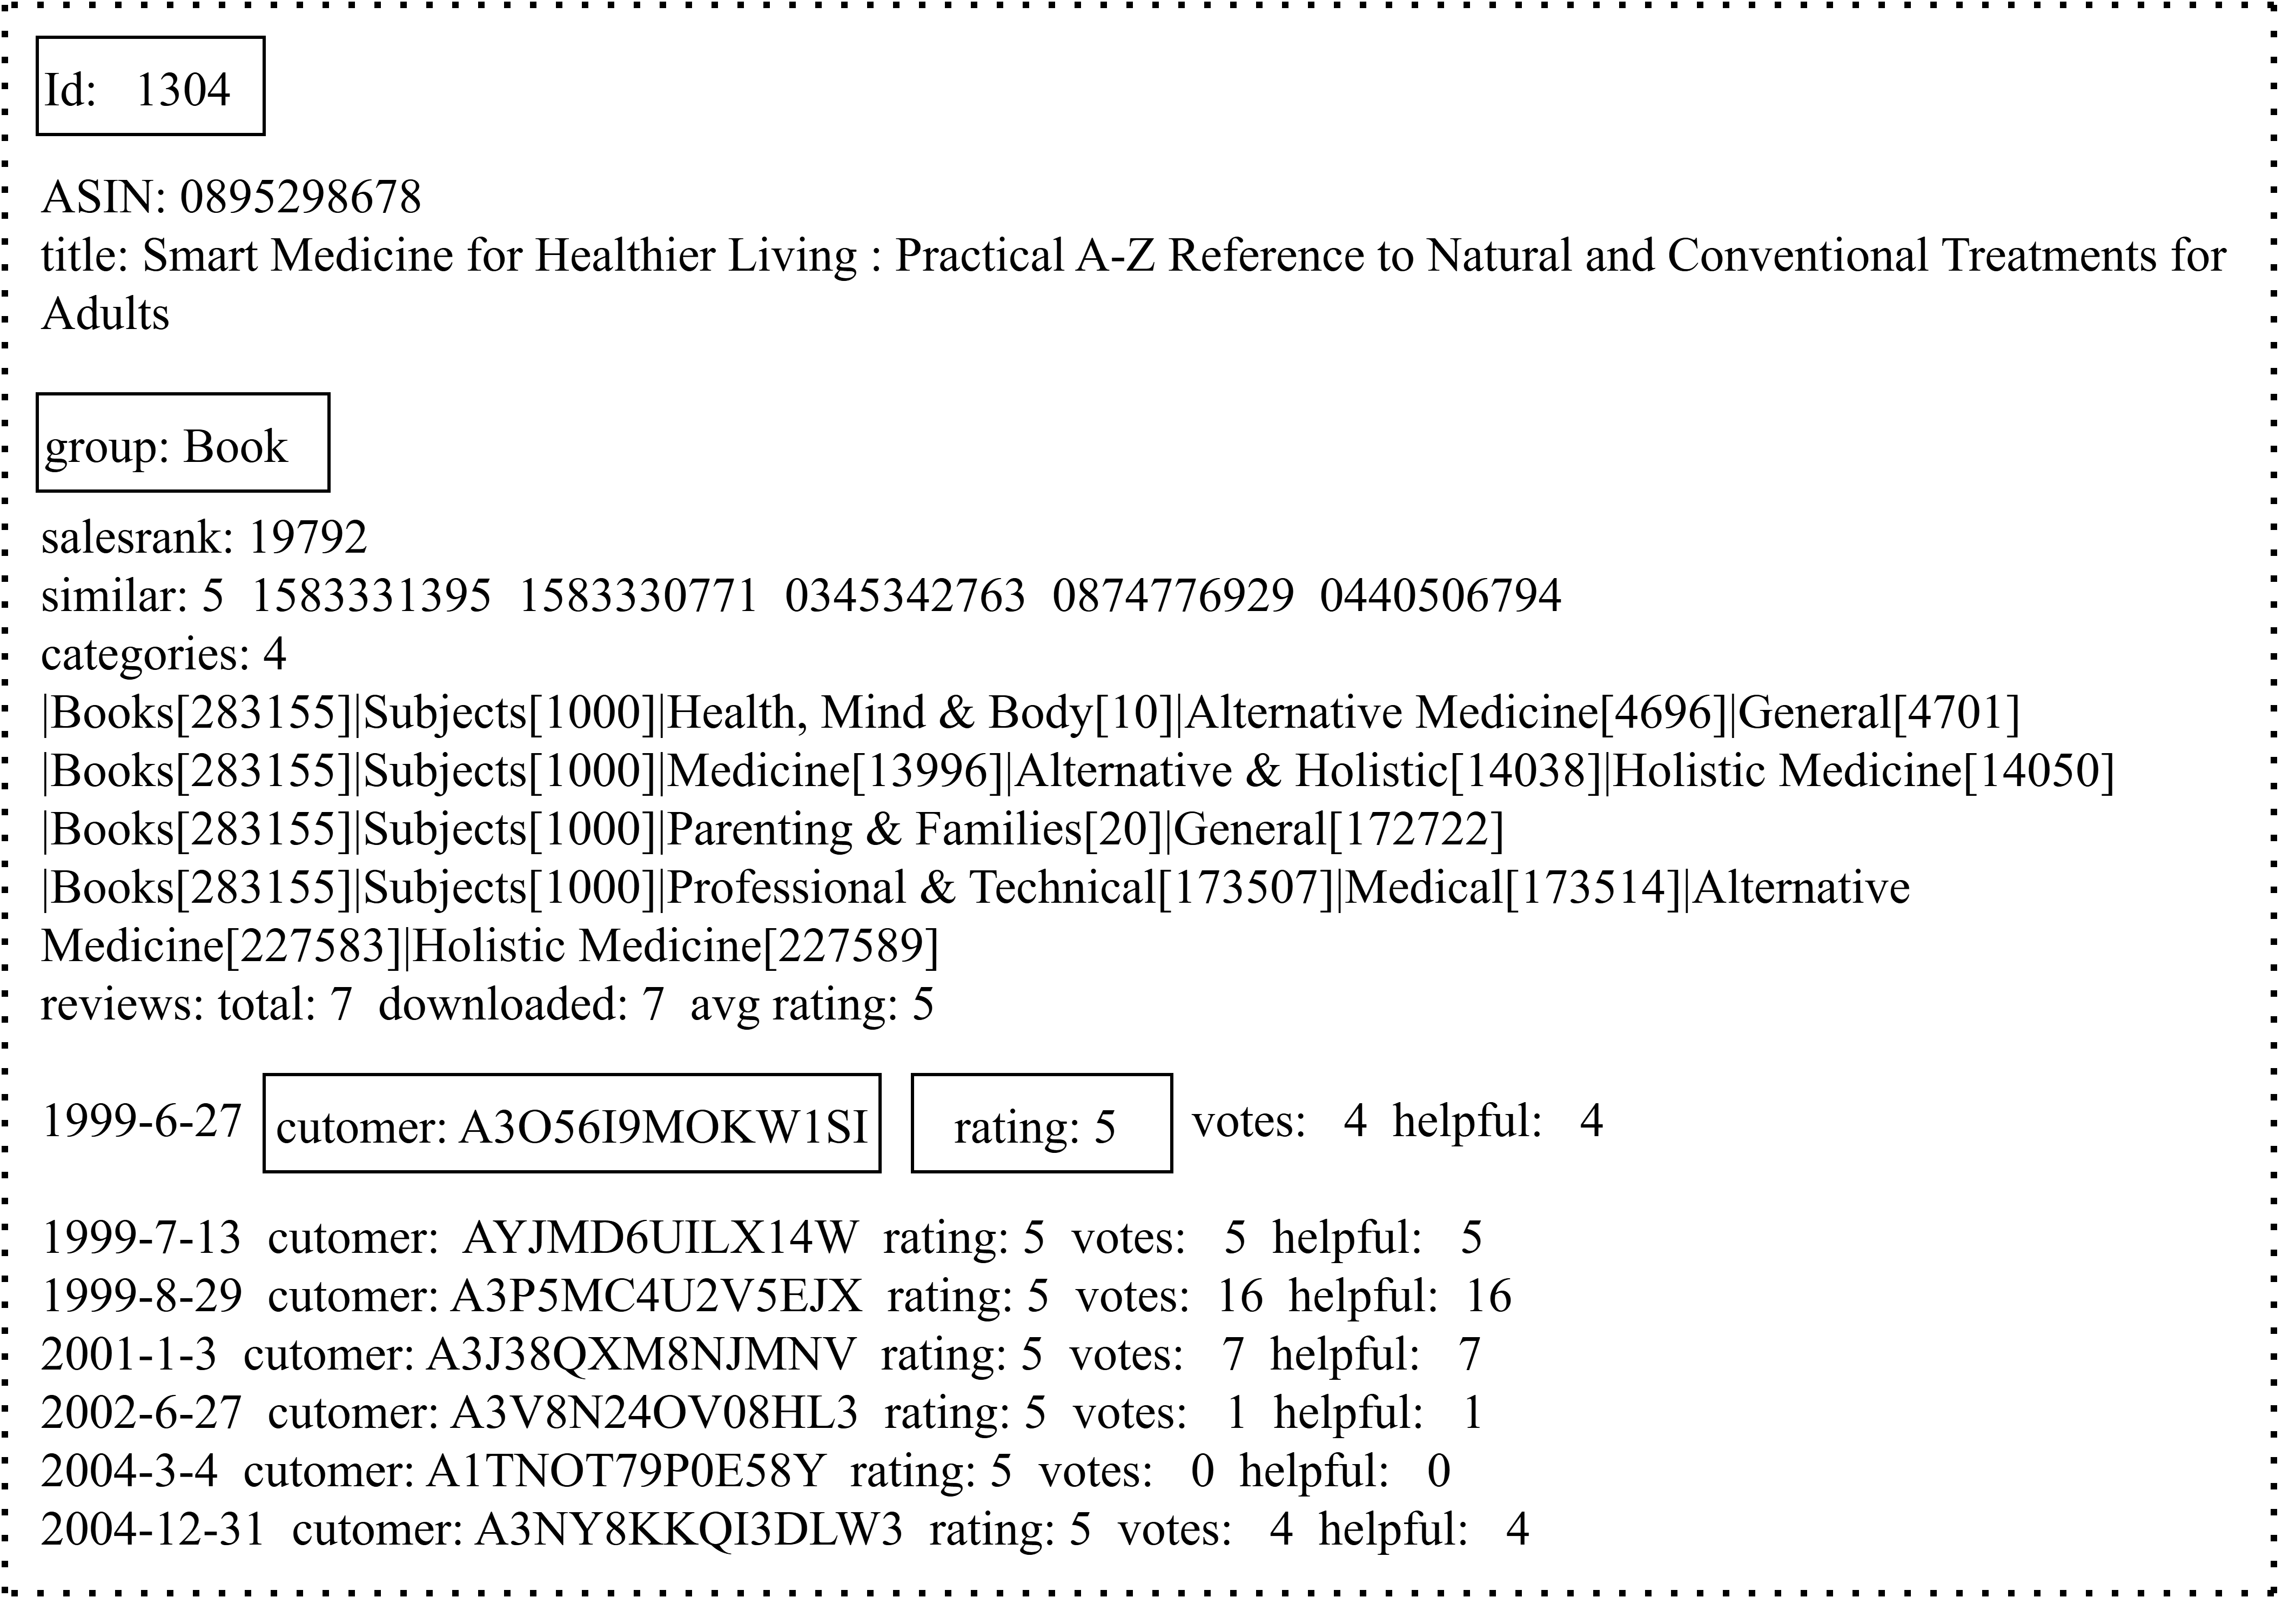
\includegraphics[width=0.8\textwidth]{Fig 6.png} 
    \caption{Amazon dataset format.}
    \label{fig:amazon_format}
\end{figure}

\subsection{Data pre-processing}


For each of our experiments in our CDRS framework we matched a ``source" domain to a ``target" domain. For each of these domains, we create a 2D rating matrix $R$, where row values indicate user ID's (users), column values indicate an item ID (items) and each cell value represents a user's rating on that particular item. There are four categories, the total number of possible category combinations is:


\begin{equation}
\binom{4}{2} = \frac{4!}{2!(4-2)!} = 6
\end{equation}

For each combination, we focused on users who engaged with both categories and provided at least 30 ratings. The minimum-30 filter is used so that each retained user has enough history for stable cross-validation splits at all training ratios (20\%--80\%); it removes extremely sparse users and therefore yields denser matrices than the raw Amazon dumps, which should be kept in mind when interpreting absolute density values. Each combination is referred to as a CDRS dataset $CX_k$, specifically $CX_1, CX_2, CX_3, CX_4, CX_5,$ and $CX_6$. We determine the source and target domains based on data density, selecting the denser dataset as the source domain and the sparser one as the target domain. All six pairs follow the \textbf{user-overlap} scenario (shared users, disjoint item sets), which is natural for Amazon category pairs where the same customers rate different product types. Item-overlap and no-overlap settings are not evaluated here and are left to future work; conclusions should therefore not be assumed to generalize automatically to those scenarios. Table \ref{tab:dataset_desc} provides the overall description of the processed dataset.

\begin{table}[ht]
\centering
\caption{Description of processed dataset}
\label{tab:dataset_desc}
\renewcommand{\arraystretch}{1.2} % Row height badhane ke liye (aapke syntax jaisa)
\setlength{\tabcolsep}{3pt} % Column spacing adjust karne ke liye taaki page se bahar na jaye
\small % Font size chhota kiya taaki table width me fit ho jaye
\begin{tabular}{lcccccc}
\hline
 & \textbf{$CX_1$} & \textbf{$CX_2$} & \textbf{$CX_3$} & \textbf{$CX_4$} & \textbf{$CX_5$} & \textbf{$CX_6$} \\
\hline
\textbf{Source Domain (S)} & Book & DVD & Video & DVD & Video & DVD \\
Users & 676 & 936 & 911 & 561 & 542 & 2020 \\
Items & 117858 & 12244 & 14978 & 11425 & 14070 & 13593 \\
Ratings & 472246 & 129581 & 134168 & 99715 & 104701 & 212353 \\
Density & 0.0059 & 0.0113 & 0.0098 & 0.0155 & 0.0137 & 0.0077 \\
\hline
\textbf{Target Domain (T)} & Music & Book & Book & Music & Music & Video \\
Users & 676 & 936 & 911 & 561 & 542 & 2020 \\
Items & 41356 & 124213 & 124188 & 39353 & 38893 & 15822 \\
Ratings & 156539 & 530461 & 526170 & 154001 & 152015 & 211850 \\
Density & 0.0055 & 0.0045 & 0.00461 & 0.0069 & 0.00721 & 0.0066 \\
\hline
\end{tabular}
\end{table}

The target densities in Table \ref{tab:dataset_desc} are all well below 1\%. Amazon category pairs are a widely used public benchmark for multi-domain recommendation with explicit ratings~\cite{he2016ups}, which motivates their use here; however, findings may not transfer unchanged to denser platforms or to domains with different feedback types.


\subsection{Implementation Details}
Experiments were run in Google Colab on a CPU High-RAM runtime (typically Intel Xeon-class host CPUs with approximately 25~GB RAM available to the notebook). Software: Python~3.x with NumPy and Scikit-learn as used in Colab at the time of the experiments. All folds used a fixed random seed of $42$ for split generation unless otherwise noted, and each method was trained for $E=20$ iterations under the shared hyperparameter setting in Section~\ref{sec:params}.

\subsection{Runtime comparison}\label{sec:runtime}
Table~\ref{tab:runtime} reports wall-clock time for a single $CX_1$ run (Book$\to$Music, 20\% target training, $E=20$ source and target, seed $42$) under the matched protocol. Absolute seconds depend on the host CPU; the useful signal is the relative cost. Rating-wise SGD methods (MF, MFB, DMF) dominate runtime: MFB is only modestly slower than MF ($\approx 118$\,s vs.\ $\approx 105$\,s) despite the extra bias parameters, while DMF is the slowest ($\approx 147$\,s) because of the element-wise product and final-layer updates. NMF's multiplicative updates and truncated-SVD warm-start finish much faster on this matrix size ($\approx 5.5$\,s and $\approx 14.9$\,s) because they are dominated by dense/sparse linear algebra rather than Python-level loops over ratings. Combined with Table~\ref{tab:method_compare}, MFB therefore offers the best accuracy--cost trade-off among the SGD family: near-MF cost with substantially lower error in the main tables.

\begin{table}[htbp]
\centering
\caption{Wall-clock runtime on $CX_1$ (one fold, TR\,$=$\,20\%, $E=20$).}
\label{tab:runtime}
\renewcommand{\arraystretch}{1.15}
\small
\begin{tabular}{lccc}
\toprule
\textbf{Method} & \textbf{Total (s)} & \textbf{s / epoch budget} & \textbf{Notes} \\
\midrule
MF\_CDRS & $105.4$ & $5.27$ & Sparse SGD \\
MFB\_CDRS & $118.2$ & $5.91$ & Sparse SGD $+$ biases \\
NMF\_CDRS & $5.5$ & $0.27$ & Multiplicative updates \\
SVD\_CDRS & $14.9$ & $0.74$ & Truncated SVD $+$ target SGD \\
DMF\_CDRS & $147.3$ & $7.36$ & GMF-style SGD \\
\bottomrule
\end{tabular}
\end{table}

\subsection{Experiment Parameter Settings and Protocols}\label{sec:params}
We used 5-fold cross-validation so that each compared method is evaluated on the same held-out partitions. For each fold, four subsets form the training data and the remaining subset is the test data. We report mean MAE/RMSE over the five folds together with a 95\% confidence interval.

To evaluate the robustness of recommendation systems over different levels of data sparseness, we partitioned the training data into 4 portions (20\%, 40\%, 60\% \& 80\%) to analyze the effects of data sparseness on both the predictive accuracy of the system and its ability to maintain stability when subjected to changing levels of data sparseness. These percentages are fractions of the already-filtered target training ratings available in each fold; they do not change the underlying catalogue density in Table \ref{tab:dataset_desc}, but they control how much target supervision the transfer models receive, so smaller percentages correspond to harder sparse-target learning conditions.


To ensure fairness and consistency throughout our study, we have standardized several hyperparameters among all studied techniques. These include: (i) a fixed dimensionality of $d=10$ latent factors; (ii) a fixed regularization parameter $\lambda = 0.01$; (iii) a fixed learning rate $\eta = 0.005$; and (iv) transfer trade-off $\gamma = 0.1$. The learning rate $\eta = 0.005$ was selected from preliminary runs in which substantially smaller rates slowed convergence under the shared 20-iteration budget, whereas larger rates produced unstable updates. Section~\ref{sec:sensitivity} reports a compact sensitivity check of $\gamma$ and $d$ for MFB\_CDRS on $CX_1$; $\lambda$ is held at $0.01$ for all methods to keep the matched protocol intact.

We trained source and target phases for $E=20$ iterations for every compared method. Figure~\ref{fig:convergence} shows a $CX_1$ probe (Book$\to$Music, TR\,$=$\,20\%) of test MAE/RMSE versus target-domain epochs for MF and MFB after a fixed 20-epoch source pre-train. Both curves flatten near epoch 20: MFB moves only from MAE $0.7045$ at $E=20$ to $0.7015$ at $E=30$, and MF from $3.0846$ to $3.0753$. The shared budget therefore sits at the knee of the curve for these linear methods and keeps the comparative protocol matched. The same fixed $E$ may still under-train slower-converging operators such as NMF and DMF; comparisons should be read as controlled under a matched protocol rather than as proof that those methods are intrinsically weaker.

\begin{figure}[htbp]
\centering
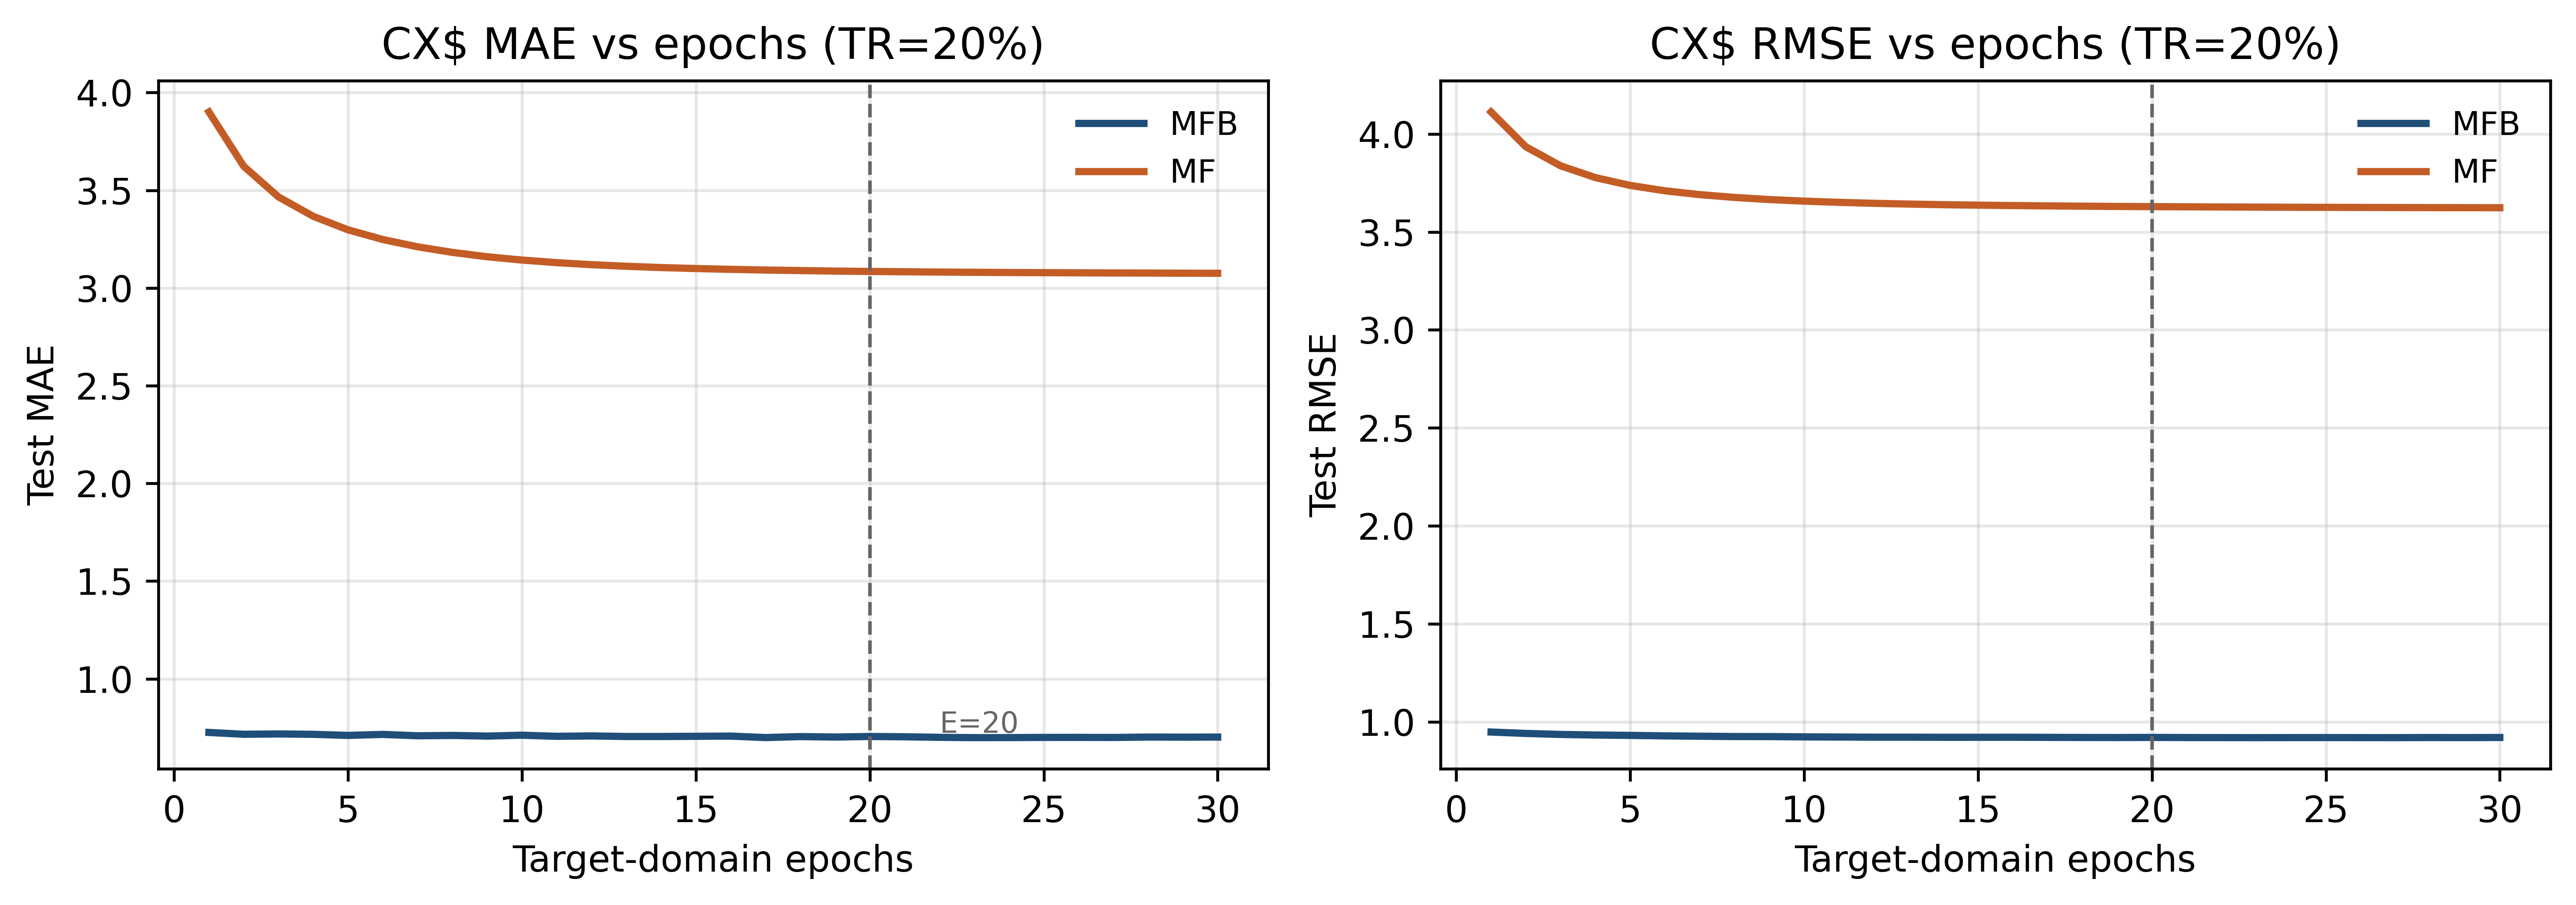
\includegraphics[width=0.95\textwidth]{Fig_convergence_cx1.png}
\caption{Target-domain convergence on $CX_1$ (TR\,$=$\,20\%). Dashed line marks the paper budget $E=20$.}
\label{fig:convergence}
\end{figure}

\subsection{Evaluation Metrics}
All observed ratings lie on a $1$--$5$ star scale. In order to determine how accurate the rating predictions are of all six of the different algorithms, we measured them via their mean absolute error (MAE) and root mean squared error (RMSE). As a trivial reference, we also include a \emph{global-mean} ($\mu$-only) baseline that predicts every test rating by the mean of the observed training ratings in that fold (no latent factors). This baseline gauges how much of each method's error is explained by predicting near the skewed Amazon rating mean.

\begin{equation}
MAE = \frac{1}{|r_T|} \sum_{(u,i) \in r_T} |r_{u,i} - \hat{r}_{u,i}|
\end{equation}

\begin{equation}
RMSE = \sqrt{\frac{1}{|r_T|} \sum_{(u,i) \in r_T} (r_{u,i} - \hat{r}_{u,i})^2}
\end{equation}

Here, $r_T$ represents the total number of ratings we predict in the target domain, $r_{u,i}$ is the actual rating provided by user $u$ for item $i$, and $\hat{r}_{u,i}$ is our predicted rating. Lower MAE or RMSE values correspond to better predictive performance. The present comparative study is restricted to this \emph{rating-prediction} setting. Ranking-oriented metrics (e.g., Precision@$K$, Recall@$K$, F1, NDCG@$K$, AUC/HR) and full-catalogue top-$N$ evaluation are left to future work when the same decompositions are assessed under an explicit ranking protocol.

\subsection{Result Analysis and Discussion}
The comprehensive experimental results are detailed in Tables \ref{tab:mae_cx1}--\ref{tab:rmse_cx6} and visualized in Fig. \ref{fig:rmse_all} and Fig. \ref{fig:mae_all}. The comparative analysis reveals distinct performance hierarchies among the decomposition approaches, providing critical insights into their intrinsic transfer capabilities.

% Figure 7 RMSE 
\begin{figure}[ht]
    \centering \includegraphics[width=0.8\textwidth]{Fig.7.png}
    \caption{RMSE of the five compared decompositions across training ratios 20\%--80\% on $CX_1$--$CX_6$ (lower is better).}
    \label{fig:rmse_all}
\end{figure}

% Figure 8 MAE
\begin{figure}[ht]
    \centering
    \includegraphics[width=0.9\textwidth]{MAE(CX1-CX6).png}
    \caption{MAE of the five compared decompositions across training ratios 20\%--80\% on $CX_1$--$CX_6$ (lower is better).}
    \label{fig:mae_all}
\end{figure}

MFB\_CDRS is always the top performer with respect to all datasets and sparsity levels. Therefore, our research shows empirical evidence to support our initial hypothesis about the inherent nature of the bias of users. When there is high sparsity of data, the signal of latent interaction between items and users can be very weak or noisy. However, the direct transfer of the user bias terms (i.e., a user's tendency to be either overly positive or overly negative), acts as a "stable anchor" that allows for stable prediction regardless of how difficult it is to learn the item specific preferences, thus providing empirical evidence of our second contribution, and demonstrating that the mechanism of transferring bias can mitigate the impact of the cold start effect.

Standard MF\_CDRS does provide very good performance as the amount of available training data increases; however, there is a noticeable drop in performance at higher sparsity levels, which again supports the need for modeling of user bias. As opposed to MF\_CDRS, the performance of SVD\_CDRS is relatively mediocre, and generally fails to better the regularization based MF and MFB models. Although the use of SVD to initialize the warm-start is theoretically correct, the empirical results indicate that the continuous regularization term employed by MF and MFB, which continuously guides the target factors toward the source factors during training, is an effective method for retaining knowledge from the source domain as opposed to simply using a single initialization.

As for non-linear and constrained methods, DMF\_CDRS, employing a neural architecture, demonstrated stable yet average performance. Although DMF\_CDRS can capture non-linear relationships between the features, it cannot compete with the linear bias-aware model under the matched protocol used here. This may partly reflect limited training budget and sparsity, rather than an intrinsic limitation of all non-linear methods. Lastly, NMF\_CDRS consistently yielded the largest errors. The constraint on non-negative values is advantageous for interpretability in single domain applications; however, in cross-domain transfer, this constraint causes significant hindrance to the model's ability to flexibly align the latent spaces of the source and target domains, resulting in negative transfer.

Overall, the above analysis unambiguously establishes that approaches that explicitly model and transfer latent user-item biases (MFB\_CDRS) provide the best means for solving the problem of cross-domain recommendations, and that these models significantly outperform both complex neural networks and constrained additive models in sparse settings.

\subsection{Ablation: bias modelling vs.\ bias transfer}\label{sec:ablation}
A natural question is whether MFB's gains come from (i)~having user/item bias parameters at all or (ii)~the $\gamma$-regularized transfer of those biases from the source. Table~\ref{tab:mae_cx1} already provides the primary ablation of (i): on $CX_1$ at 20\% training, removing biases entirely (MF\_CDRS) raises MAE from $0.6834$ (MFB) to $3.6606$. Table~\ref{tab:ablation} isolates (ii) on the same $CX_1$ split used for the runtime probe (TR\,$=$\,20\%, $E=20$): MFB with factor transfer only (biases fitted locally, no $\gamma$ pull on $b_u,b_i$) matches full bias+factor transfer to three decimals (MAE $0.6922$ vs.\ $0.6930$), while MF without biases remains far worse ($3.0626$ on this probe). Thus, under the matched sparse protocol, the decisive ingredient is \emph{modelling} biases in the predictor; continuous bias-alignment adds little once local biases are free parameters. This clarifies the mechanism behind MFB's MAE/RMSE advantage without claiming that $\gamma$ bias transfer is universally necessary.

\begin{table}[htbp]
\centering
\caption{Bias ablation on $CX_1$ (one fold, TR\,$=$\,20\%, $E=20$).}
\label{tab:ablation}
\renewcommand{\arraystretch}{1.15}
\small
\begin{tabular}{lc}
\toprule
\textbf{Variant} & \textbf{MAE} \\
\midrule
MF (no bias parameters) & $3.0626$ \\
MFB, factor transfer only (local biases) & $0.6922$ \\
MFB, full (factor $+$ bias transfer) & $0.6930$ \\
\bottomrule
\end{tabular}
\end{table}

\subsection{Cold-start user slices and rating-bin errors}\label{sec:coldstart}
To address requests for finer-grained evaluation beyond overall MAE, Table~\ref{tab:coldstart} splits $CX_1$ test users (TR\,$=$\,20\%) into cold / mid / warm terciles by the number of target training ratings (cut-offs 7 and 15). MFB remains best in every slice (cold MAE $0.689$ vs.\ DMF $0.766$ and $\mu$ $0.777$), so the comparative ranking is not driven only by warm users. Table~\ref{tab:rating_bins} further breaks test errors by true rating value. Absolute errors are largest on rare low ratings ($1$--$2$), where MFB still improves over $\mu$ and DMF; on the dominant high ratings ($4$--$5$) all methods are closer, and MFB retains a small edge. These component views support the same comparative conclusion as the aggregate tables without introducing a new model.

\begin{table}[htbp]
\centering
\caption{Per-user MAE on $CX_1$ by target-training activity (TR\,$=$\,20\%).}
\label{tab:coldstart}
\renewcommand{\arraystretch}{1.15}
\small
\begin{tabular}{lcccc}
\toprule
\textbf{Slice} & \textbf{Users} & $\mu$ & MFB & DMF \\
\midrule
Cold ($\le 7$ train ratings) & 227 & $0.777$ & $0.689$ & $0.766$ \\
Mid & 220 & $0.771$ & $0.678$ & $0.761$ \\
Warm ($> 15$ train ratings) & 203 & $0.808$ & $0.687$ & $0.804$ \\
\bottomrule
\end{tabular}
\end{table}

\begin{table}[htbp]
\centering
\caption{Component MAE on $CX_1$ test ratings by true rating bin (TR\,$=$\,20\%).}
\label{tab:rating_bins}
\renewcommand{\arraystretch}{1.15}
\small
\begin{tabular}{lcccc}
\toprule
\textbf{True rating} & \textbf{$n$} & $\mu$ & MFB & DMF \\
\midrule
Low ($1$--$2$) & 1075 & $2.783$ & $2.332$ & $2.824$ \\
Mid ($3$) & 1819 & $1.324$ & $1.112$ & $1.365$ \\
High ($4$--$5$) & 15839 & $0.558$ & $0.518$ & $0.539$ \\
\bottomrule
\end{tabular}
\end{table}

\subsection{Relation to stronger CDRS systems}
This paper is a comparative evaluation of foundational decompositions, not a proposal of a new CDRS architecture and not a claim to beat recent graph, adversarial, or sequential systems on their native benchmarks. Those systems typically optimize ranking losses on denser or sequential logs and add substantial machinery around an embedding backbone (Table~\ref{tab:related_work_summary}). Under the matched sparse \emph{rating-prediction} protocol studied here, bias-aware factorization (MFB) is simply the strongest among the five compared operators---and stronger than a $\mu$ baseline---on MAE/RMSE. The practical takeaway for comparative CDRS work is therefore methodological: when reporting gains from deeper models in sparse targets, an MFB-style bias-aware transfer baseline is a fair reference point for the decomposition component. Ranking-protocol comparisons against those systems are future work.

\subsection{Hyperparameter sensitivity}\label{sec:sensitivity}
To make the shared hyperparameter choice transparent, Table~\ref{tab:sensitivity} reports an MFB\_CDRS sensitivity probe on $CX_1$ (Book$\to$Music) at 20\% target training with the same seed ($42$) and $E=20$ budget as the main protocol (one held-out fold for this probe; the comparative MAE/RMSE tables remain 5-fold). Varying $\gamma\in\{0,0.01,0.1,1\}$ at $d=10$ leaves MAE essentially unchanged at full budget ($0.7378$), indicating that---under user-overlap transfer with matched epochs---final rating error is robust to the precise transfer weight once target SGD has run. Mid-training snapshots can still separate $\gamma$ values, but the operating point used in the paper is insensitive. Varying $d\in\{5,10,20\}$ at $\gamma=0.1$ shows a mild preference for the smaller latent size ($d=5$: $0.7280$; $d=10$: $0.7378$; $d=20$: $0.7396$). We retain $d=10$ in the main tables as a shared setting across MF/MFB/NMF/DMF/SVD that balances capacity and cost; the probe does not support claiming that larger $d$ helps under this sparse target protocol.

\begin{table}[htbp]
\centering
\caption{MFB\_CDRS sensitivity on $CX_1$ at 20\% training ($E=20$, seed $42$).}
\label{tab:sensitivity}
\renewcommand{\arraystretch}{1.15}
\small
\begin{tabular}{lcc}
\toprule
\textbf{Setting} & \textbf{Value} & \textbf{MAE} \\
\midrule
$\gamma$ ($d=10$) & $0.0$ / $0.01$ / $0.1$ / $1.0$ & $0.7378$ / $0.7378$ / $0.7378$ / $0.7378$ \\
$d$ ($\gamma=0.1$) & $5$ / $10$ / $20$ & $0.7280$ / $0.7378$ / $0.7396$ \\
\bottomrule
\end{tabular}
\end{table}

\subsection{Global-mean ($\mu$) baseline}
Because Amazon ratings are strongly skewed toward high scores (overall mean $\approx 4.18$ on the $1$--$5$ scale in our parsed dump), a trivial predictor that always outputs the training-fold mean is a necessary reference. Table~\ref{tab:mu_baseline} reports this $\mu$-only baseline under the same 5-fold protocol (seed $42$) and training ratios as the decomposition methods. At 20\% target training, $\mu$ yields MAE in the range $0.78$--$0.91$ across the six pairs. MFB\_CDRS remains clearly better than $\mu$ on every pair (e.g., $CX_2$: $0.6612$ vs.\ $0.7888$; $CX_6$: $0.7947$ vs.\ $0.9128$), so MFB's advantage is not explained by mean prediction alone. MF, SVD, and NMF remain far worse than $\mu$, which further indicates that those transfers fail to exploit even the rating mean under the matched sparse protocol.

\begin{table}[htbp]
\centering
\caption{Global-mean ($\mu$-only) baseline MAE/RMSE (mean $\pm$ 95\% CI) on target domains.}
\label{tab:mu_baseline}
\renewcommand{\arraystretch}{1.15}
\setlength{\tabcolsep}{3pt}
\small
\begin{tabular}{llcccc}
\toprule
\textbf{Pair} & \textbf{Target} & \textbf{TR 20\% MAE} & \textbf{TR 20\% RMSE} & \textbf{TR 80\% MAE} & \textbf{TR 80\% RMSE} \\
\midrule
Book--Music & Book$^{\dagger}$ & $0.7796\pm0.0003$ & $0.9635\pm0.0027$ & $0.7795\pm0.0007$ & $0.9635\pm0.0027$ \\
$CX_2$ (DVD$\to$Book) & Book & $0.7888\pm0.0016$ & $0.9778\pm0.0018$ & $0.7887\pm0.0015$ & $0.9778\pm0.0018$ \\
$CX_3$ (Video$\to$Book) & Book & $0.7876\pm0.0027$ & $0.9775\pm0.0053$ & $0.7884\pm0.0031$ & $0.9775\pm0.0052$ \\
$CX_4$ (DVD$\to$Music) & Music & $0.7892\pm0.0035$ & $1.0001\pm0.0067$ & $0.7887\pm0.0040$ & $1.0001\pm0.0067$ \\
$CX_5$ (Video$\to$Music) & Music & $0.7826\pm0.0040$ & $0.9935\pm0.0061$ & $0.7845\pm0.0033$ & $0.9934\pm0.0061$ \\
$CX_6$ (DVD$\to$Video) & Video & $0.9128\pm0.0017$ & $1.1678\pm0.0033$ & $0.9124\pm0.0015$ & $1.1677\pm0.0033$ \\
\bottomrule
\end{tabular}\\[0.3em]
\footnotesize{$^{\dagger}$On this re-parse, Music was denser than Book among overlapping users, so the $\mu$ baseline is reported on Book as the sparse target; $CX_2$--$CX_6$ match Table~\ref{tab:dataset_desc}.}
\end{table}

\subsection{Statistical significance}
To support ranking claims beyond overlapping confidence intervals, we applied paired tests on the five fold-level MAE values using the same notebook folds (seed $42$). Table~\ref{tab:sig_cx1} reports paired $t$-tests on $CX_1$ (Book$\to$Music) at 20\% target training, comparing MFB\_CDRS with each alternative. All paired $t$-tests are significant at $p<0.001$. Exact Wilcoxon signed-rank $p$-values equal $0.0625$ with $n=5$ when MFB wins every fold (the minimum attainable two-sided exact $p$ for this sample size); the directional consistency across folds nevertheless supports the ranking. The same pattern holds at 80\% training for MFB vs.\ DMF on $CX_1$ ($t=-44.77$, $p=1.5\times 10^{-6}$).

Table~\ref{tab:sig_mfb_dmf} extends the closest competitor comparison (MFB vs.\ DMF) to all six domain pairs at 20\% training: every pair yields a paired $t$-test with $p<0.001$, and MFB has lower MAE on all five folds in each pair.

\begin{table}[htbp]
\centering
\caption{Paired tests on fold-level MAE for $CX_1$ at 20\% training (MFB vs.\ alternatives).}
\label{tab:sig_cx1}
\renewcommand{\arraystretch}{1.2}
\small
\begin{tabular}{lcccc}
\toprule
\textbf{Comparison} & \textbf{Mean MAE (MFB)} & \textbf{Mean MAE (alt.)} & \textbf{Paired $t$} & \textbf{$p$ (paired $t$)} \\
\midrule
MFB vs.\ MF & 0.6834 & 3.6606 & $-303.39$ & $7.1\times 10^{-10}$ \\
MFB vs.\ NMF & 0.6834 & 4.3456 & $-666.73$ & $3.0\times 10^{-11}$ \\
MFB vs.\ DMF & 0.6834 & 0.7637 & $-12.20$ & $2.6\times 10^{-4}$ \\
MFB vs.\ SVD & 0.6834 & 3.3108 & $-101.53$ & $5.6\times 10^{-8}$ \\
\bottomrule
\end{tabular}
\end{table}

\begin{table}[htbp]
\centering
\caption{Paired $t$-tests on fold-level MAE: MFB vs.\ DMF at 20\% training across all domain pairs.}
\label{tab:sig_mfb_dmf}
\renewcommand{\arraystretch}{1.2}
\small
\begin{tabular}{lcccc}
\toprule
\textbf{Dataset} & \textbf{Mean MAE (MFB)} & \textbf{Mean MAE (DMF)} & \textbf{Paired $t$} & \textbf{$p$ (paired $t$)} \\
\midrule
$CX_1$ & 0.6834 & 0.7636 & $-12.20$ & $2.6\times 10^{-4}$ \\
$CX_2$ & 0.6612 & 0.8129 & $-34.95$ & $4.0\times 10^{-6}$ \\
$CX_3$ & 0.6611 & 0.8057 & $-18.28$ & $5.3\times 10^{-5}$ \\
$CX_4$ & 0.6875 & 0.7664 & $-21.25$ & $2.9\times 10^{-5}$ \\
$CX_5$ & 0.6869 & 0.7782 & $-19.74$ & $3.9\times 10^{-5}$ \\
$CX_6$ & 0.7947 & 0.9137 & $-114.83$ & $3.5\times 10^{-8}$ \\
\bottomrule
\end{tabular}
\end{table}

% --- DATA TABLES START HERE ---

% Table 2: MAE CX1
\begin{table}[ht]
\centering
\caption{MAE performance on the $CX_1$ dataset with four training set size}
\label{tab:mae_cx1}
\renewcommand{\arraystretch}{1.2}
\begin{tabular*}{\textwidth}{@{\extracolsep\fill}lcccc}
\toprule
\textbf{List of Approaches} & \multicolumn{4}{c}{\underline{\textbf{Training set size (TR)}}} \\
 & \textbf{20\%} & \textbf{40\%} & \textbf{60\%} & \textbf{80\%} \\
\midrule
NMF\_CDRS & $4.3456 \pm 0.0086$ & $4.3323 \pm 0.0092$ & $4.3161 \pm 0.0103$ & $4.2975 \pm 0.0115$ \\
MF\_CDRS & $3.6606 \pm 0.0177$ & $2.8952 \pm 0.0177$ & $2.4246 \pm 0.0190$ & $2.1301 \pm 0.0148$ \\
SVD\_CDRS & $3.3108 \pm 0.0432$ & $3.2019 \pm 0.0942$ & $3.1116 \pm 0.1822$ & $3.0387 \pm 0.2568$ \\
DMF\_CDRS & $0.7637 \pm 0.0168$ & $0.7954 \pm 0.0199$ & $0.8221 \pm 0.0101$ & $0.8352 \pm 0.0110$ \\
MFB\_CDRS & $0.6834 \pm 0.0037$ & $0.6698 \pm 0.0017$ & $0.6637 \pm 0.0015$ & $0.6610 \pm 0.0025$ \\
\bottomrule
\end{tabular*}
\end{table}

% Table 3: RMSE CX1
\begin{table}[ht]
\centering
\caption{RMSE performance on the $CX_1$ dataset with four training set size}
\label{tab:rmse_cx1}
\renewcommand{\arraystretch}{1.2}
\begin{tabular*}{\textwidth}{@{\extracolsep\fill}lcccc}
\toprule
\textbf{List of Approaches} & \multicolumn{4}{c}{\underline{\textbf{Training set size (TR)}}} \\
 & \textbf{20\%} & \textbf{40\%} & \textbf{60\%} & \textbf{80\%} \\
\midrule
NMF\_CDRS & $4.4511 \pm 0.0066$ & $4.4387 \pm 0.0070$ & $4.4236 \pm 0.0079$ & $4.4071 \pm 0.0085$ \\
MF\_CDRS & $3.9700 \pm 0.0118$ & $3.4083 \pm 0.0142$ & $3.0502 \pm 0.0141$ & $2.8128 \pm 0.0128$ \\
SVD\_CDRS & $3.4594 \pm 0.0305$ & $3.3885 \pm 0.0612$ & $3.3283 \pm 0.1196$ & $3.2799 \pm 0.1692$ \\
DMF\_CDRS & $0.9642 \pm 0.0119$ & $0.9814 \pm 0.0183$ & $1.0062 \pm 0.0140$ & $1.0203 \pm 0.0131$ \\
MFB\_CDRS & $0.8942 \pm 0.0055$ & $0.8829 \pm 0.0041$ & $0.8842 \pm 0.0041$ & $0.8799 \pm 0.0042$ \\
\bottomrule
\end{tabular*}
\end{table}

% Table 4: MAE CX2
\begin{table}[ht]
\centering
\caption{MAE performance on the $CX_2$ dataset with four training set size}
\label{tab:mae_cx2}
\renewcommand{\arraystretch}{1.2}
\begin{tabular*}{\textwidth}{@{\extracolsep\fill}lcccc}
\toprule
\textbf{List of Approaches} & \multicolumn{4}{c}{\underline{\textbf{Training set size (TR)}}} \\
 & \textbf{20\%} & \textbf{40\%} & \textbf{60\%} & \textbf{80\%} \\
\midrule
NMF\_CDRS & $4.3168 \pm 0.0192$ & $4.3015 \pm 0.0164$ & $4.2836 \pm 0.0152$ & $4.2565 \pm 0.0198$ \\
MF\_CDRS & $3.4285 \pm 0.0082$ & $2.8061 \pm 0.0053$ & $2.4774 \pm 0.0051$ & $2.2656 \pm 0.0048$ \\
SVD\_CDRS & $3.2804 \pm 0.0672$ & $3.1902 \pm 0.1442$ & $3.1238 \pm 0.2106$ & $3.0672 \pm 0.2691$ \\
DMF\_CDRS & $0.8129 \pm 0.0119$ & $0.8209 \pm 0.0081$ & $0.8182 \pm 0.0144$ & $0.8029 \pm 0.0096$ \\
MFB\_CDRS & $0.6612 \pm 0.0033$ & $0.6543 \pm 0.0033$ & $0.6517 \pm 0.0019$ & $0.6504 \pm 0.0032$ \\
\bottomrule
\end{tabular*}
\end{table}

% Table 5: RMSE CX2
\begin{table}[ht]
\centering
\caption{RMSE performance on the $CX_2$ dataset with four training set size}
\label{tab:rmse_cx2}
\renewcommand{\arraystretch}{1.2}
\begin{tabular*}{\textwidth}{@{\extracolsep\fill}lcccc}
\toprule
\textbf{List of Approaches} & \multicolumn{4}{c}{\underline{\textbf{Training set size (TR)}}} \\
 & \textbf{20\%} & \textbf{40\%} & \textbf{60\%} & \textbf{80\%} \\
\midrule
NMF\_CDRS & $4.4197 \pm 0.0153$ & $4.4051 \pm 0.0127$ & $4.3881 \pm 0.0115$ & $4.3628 \pm 0.0156$ \\
MF\_CDRS & $3.8153 \pm 0.0070$ & $3.3833 \pm 0.0046$ & $3.1391 \pm 0.0049$ & $2.9682 \pm 0.0041$ \\
SVD\_CDRS & $3.4338 \pm 0.0562$ & $3.3761 \pm 0.1022$ & $3.3341 \pm 0.1431$ & $3.2997 \pm 0.1779$ \\
DMF\_CDRS & $0.9943 \pm 0.0143$ & $1.0029 \pm 0.0107$ & $0.9990 \pm 0.0159$ & $0.9837 \pm 0.0108$ \\
MFB\_CDRS & $0.9011 \pm 0.0034$ & $0.8909 \pm 0.0041$ & $0.8842 \pm 0.0041$ & $0.8799 \pm 0.0042$ \\
\bottomrule
\end{tabular*}
\end{table}

% Table 6: MAE CX3
\begin{table}[ht]
\centering
\caption{MAE performance on the $CX_3$ dataset with four training set size}
\label{tab:mae_cx3}
\renewcommand{\arraystretch}{1.2}
\begin{tabular*}{\textwidth}{@{\extracolsep\fill}lcccc}
\toprule
\textbf{List of Approaches} & \multicolumn{4}{c}{\underline{\textbf{Training set size (TR)}}} \\
 & \textbf{20\%} & \textbf{40\%} & \textbf{60\%} & \textbf{80\%} \\
\midrule
NMF\_CDRS & $4.3188 \pm 0.0037$ & $4.3070 \pm 0.0048$ & $4.2899 \pm 0.0074$ & $4.2696 \pm 0.0119$ \\
MF\_CDRS & $3.4519 \pm 0.0089$ & $2.8355 \pm 0.0051$ & $2.5119 \pm 0.0044$ & $2.3011 \pm 0.0068$ \\
SVD\_CDRS & $3.2779 \pm 0.0715$ & $3.1885 \pm 0.1503$ & $3.1176 \pm 0.2189$ & $3.0614 \pm 0.2763$ \\
DMF\_CDRS & $0.8056 \pm 0.0184$ & $0.8081 \pm 0.0095$ & $0.8067 \pm 0.0107$ & $0.8006 \pm 0.0107$ \\
MFB\_CDRS & $0.6611 \pm 0.0015$ & $0.6541 \pm 0.0019$ & $0.6516 \pm 0.0022$ & $0.6516 \pm 0.0020$ \\
\bottomrule
\end{tabular*}
\end{table}

% Table 7: RMSE CX3
\begin{table}[ht]
\centering
\caption{RMSE performance on the $CX_3$ dataset with four training set size}
\label{tab:rmse_cx3}
\renewcommand{\arraystretch}{1.2}
\begin{tabular*}{\textwidth}{@{\extracolsep\fill}lcccc}
\toprule
\textbf{List of Approaches} & \multicolumn{4}{c}{\underline{\textbf{Training set size (TR)}}} \\
 & \textbf{20\%} & \textbf{40\%} & \textbf{60\%} & \textbf{80\%} \\
\midrule
NMF\_CDRS & $4.4226 \pm 0.0035$ & $4.4115 \pm 0.0042$ & $4.3951 \pm 0.0069$ & $4.3763 \pm 0.0109$ \\
MF\_CDRS & $3.8352 \pm 0.0070$ & $3.4092 \pm 0.0052$ & $3.1674 \pm 0.0033$ & $2.9993 \pm 0.0075$ \\
SVD\_CDRS & $3.4318 \pm 0.0603$ & $3.3745 \pm 0.1077$ & $3.3299 \pm 0.1494$ & $3.2957 \pm 0.1840$ \\
DMF\_CDRS & $0.9873 \pm 0.0204$ & $0.9889 \pm 0.0119$ & $0.9877 \pm 0.0128$ & $0.9819 \pm 0.0118$ \\
MFB\_CDRS & $0.9006 \pm 0.0040$ & $0.8907 \pm 0.0036$ & $0.8840 \pm 0.0035$ & $0.8796 \pm 0.0027$ \\
\bottomrule
\end{tabular*}
\end{table}

% Table 8: MAE CX4
\begin{table}[ht]
\centering
\caption{MAE performance on the $CX_4$ dataset with four training set size}
\label{tab:mae_cx4}
\renewcommand{\arraystretch}{1.2}
\begin{tabular*}{\textwidth}{@{\extracolsep\fill}lcccc}
\toprule
\textbf{List of Approaches} & \multicolumn{4}{c}{\underline{\textbf{Training set size (TR)}}} \\
 & \textbf{20\%} & \textbf{40\%} & \textbf{60\%} & \textbf{80\%} \\
\midrule
NMF\_CDRS & $4.4159 \pm 0.0121$ & $4.3878 \pm 0.0143$ & $4.3530 \pm 0.0143$ & $4.3127 \pm 0.0152$ \\
MF\_CDRS & $3.6213 \pm 0.0079$ & $2.8263 \pm 0.0054$ & $2.3937 \pm 0.0089$ & $2.1207 \pm 0.0061$ \\
SVD\_CDRS & $3.2866 \pm 0.0523$ & $3.1790 \pm 0.0972$ & $3.0958 \pm 0.1759$ & $3.0278 \pm 0.2426$ \\
DMF\_CDRS & $0.7664 \pm 0.0077$ & $0.7844 \pm 0.0037$ & $0.7948 \pm 0.0099$ & $0.7994 \pm 0.0118$ \\
MFB\_CDRS & $0.6875 \pm 0.0016$ & $0.6727 \pm 0.0026$ & $0.6668 \pm 0.0018$ & $0.6632 \pm 0.0025$ \\
\bottomrule
\end{tabular*}
\end{table}

% Table 9: RMSE CX4
\begin{table}[ht]
\centering
\caption{RMSE performance on the $CX_4$ dataset with four training set size}
\label{tab:rmse_cx4}
\renewcommand{\arraystretch}{1.2}
\begin{tabular*}{\textwidth}{@{\extracolsep\fill}lcccc}
\toprule
\textbf{List of Approaches} & \multicolumn{4}{c}{\underline{\textbf{Training set size (TR)}}} \\
 & \textbf{20\%} & \textbf{40\%} & \textbf{60\%} & \textbf{80\%} \\
\midrule
NMF\_CDRS & $4.5048 \pm 0.0101$ & $4.4790 \pm 0.0119$ & $4.4481 \pm 0.0125$ & $4.4126 \pm 0.0122$ \\
MF\_CDRS & $3.9340 \pm 0.0054$ & $3.3526 \pm 0.0061$ & $3.0238 \pm 0.0083$ & $2.7983 \pm 0.0066$ \\
SVD\_CDRS & $3.4466 \pm 0.0385$ & $3.3777 \pm 0.0657$ & $3.3235 \pm 0.1160$ & $3.2792 \pm 0.1585$ \\
DMF\_CDRS & $0.9901 \pm 0.0046$ & $0.9922 \pm 0.0038$ & $0.9968 \pm 0.0039$ & $0.9992 \pm 0.0045$ \\
MFB\_CDRS & $0.9163 \pm 0.0054$ & $0.9040 \pm 0.0059$ & $0.8984 \pm 0.0057$ & $0.8936 \pm 0.0059$ \\
\bottomrule
\end{tabular*}
\end{table}

% Table 10: MAE CX5
\begin{table}[ht]
\centering
\caption{MAE performance on the $CX_5$ dataset with four training set size}
\label{tab:mae_cx5}
\renewcommand{\arraystretch}{1.2}
\begin{tabular*}{\textwidth}{@{\extracolsep\fill}lcccc}
\toprule
\textbf{List of Approaches} & \multicolumn{4}{c}{\underline{\textbf{Training set size (TR)}}} \\
 & \textbf{20\%} & \textbf{40\%} & \textbf{60\%} & \textbf{80\%} \\
\midrule
NMF\_CDRS & $4.4220 \pm 0.0107$ & $4.3909 \pm 0.0100$ & $4.3587 \pm 0.0102$ & $4.3174 \pm 0.0110$ \\
MF\_CDRS & $3.6235 \pm 0.0136$ & $2.8391 \pm 0.0123$ & $2.4008 \pm 0.0188$ & $2.1230 \pm 0.0117$ \\
SVD\_CDRS & $3.2926 \pm 0.0555$ & $3.1779 \pm 0.0831$ & $3.0913 \pm 0.1604$ & $3.0269 \pm 0.2214$ \\
DMF\_CDRS & $0.7782 \pm 0.0176$ & $0.7862 \pm 0.0233$ & $0.7971 \pm 0.0181$ & $0.8057 \pm 0.0113$ \\
MFB\_CDRS & $0.6868 \pm 0.0068$ & $0.6750 \pm 0.0063$ & $0.6695 \pm 0.0080$ & $0.6635 \pm 0.0052$ \\
\bottomrule
\end{tabular*}
\end{table}

% Table 11: RMSE CX5
\begin{table}[ht]
\centering
\caption{RMSE performance on the $CX_5$ dataset with four training set size}
\label{tab:rmse_cx5}
\renewcommand{\arraystretch}{1.2}
\begin{tabular*}{\textwidth}{@{\extracolsep\fill}lcccc}
\toprule
\textbf{List of Approaches} & \multicolumn{4}{c}{\underline{\textbf{Training set size (TR)}}} \\
 & \textbf{20\%} & \textbf{40\%} & \textbf{60\%} & \textbf{80\%} \\
\midrule
NMF\_CDRS & $4.5097 \pm 0.0082$ & $4.4818 \pm 0.0076$ & $4.4526 \pm 0.0078$ & $4.4160 \pm 0.0096$ \\
MF\_CDRS & $3.9384 \pm 0.0107$ & $3.3653 \pm 0.0099$ & $3.0317 \pm 0.0175$ & $2.8028 \pm 0.0122$ \\
SVD\_CDRS & $3.4519 \pm 0.0413$ & $3.3771 \pm 0.0561$ & $3.3211 \pm 0.1035$ & $3.2796 \pm 0.1420$ \\
DMF\_CDRS & $0.9903 \pm 0.0126$ & $0.9931 \pm 0.0157$ & $0.9967 \pm 0.0159$ & $1.0013 \pm 0.0121$ \\
MFB\_CDRS & $0.9185 \pm 0.0094$ & $0.9056 \pm 0.0083$ & $0.8994 \pm 0.0095$ & $0.8956 \pm 0.0073$ \\
\bottomrule
\end{tabular*}
\end{table}

% Table 12: MAE CX6 (Set 1)
\begin{table}[ht]
\centering
\caption{MAE performance on the $CX_6$ dataset with four training set size}
\label{tab:mae_cx6}
\renewcommand{\arraystretch}{1.2}
\begin{tabular*}{\textwidth}{@{\extracolsep\fill}lcccc}
\toprule
\textbf{List of Approaches} & \multicolumn{4}{c}{\underline{\textbf{Training set size (TR)}}} \\
 & \textbf{20\%} & \textbf{40\%} & \textbf{60\%} & \textbf{80\%} \\
\midrule
NMF\_CDRS & $4.0645 \pm 0.0035$ & $4.0268 \pm 0.0041$ & $3.9818 \pm 0.0118$ & $3.9307 \pm 0.0167$ \\
MF\_CDRS & $2.0973 \pm 0.0054$ & $1.3021 \pm 0.0083$ & $1.0843 \pm 0.0076$ & $0.9825 \pm 0.0081$ \\
SVD\_CDRS & $3.0386 \pm 0.0215$ & $3.0280 \pm 0.0254$ & $3.0230 \pm 0.0289$ & $3.0211 \pm 0.0301$ \\
DMF\_CDRS & $0.9137 \pm 0.0009$ & $0.9136 \pm 0.0011$ & $0.9130 \pm 0.0015$ & $0.9122 \pm 0.0012$ \\
MFB\_CDRS & $0.7947 \pm 0.0021$ & $0.7630 \pm 0.0024$ & $0.7476 \pm 0.0019$ & $0.7372 \pm 0.0021$ \\
\bottomrule
\end{tabular*}
\end{table}

% Table 13: RMSE CX6 (Set 2)
\begin{table}[ht]
\centering
\caption{RMSE performance on the $CX_6$ dataset with four training set size}
\label{tab:rmse_cx6}
\renewcommand{\arraystretch}{1.2}
\begin{tabular*}{\textwidth}{@{\extracolsep\fill}lcccc}
\toprule
\textbf{List of Approaches} & \multicolumn{4}{c}{\underline{\textbf{Training set size (TR)}}} \\
 & \textbf{20\%} & \textbf{40\%} & \textbf{60\%} & \textbf{80\%} \\
\midrule
NMF\_CDRS & $4.2222 \pm 0.0021$ & $4.1861 \pm 0.0033$ & $4.1441 \pm 0.0098$ & $4.0976 \pm 0.0135$ \\
MF\_CDRS & $2.5666 \pm 0.0054$ & $1.7928 \pm 0.0112$ & $1.5425 \pm 0.0101$ & $1.4108 \pm 0.0115$ \\
SVD\_CDRS & $3.2570 \pm 0.0153$ & $3.2506 \pm 0.0166$ & $3.2479 \pm 0.0181$ & $3.2469 \pm 0.0184$ \\
DMF\_CDRS & $1.1714 \pm 0.0016$ & $1.1711 \pm 0.0033$ & $1.1704 \pm 0.0029$ & $1.1689 \pm 0.0020$ \\
MFB\_CDRS & $1.0291 \pm 0.0028$ & $0.9992 \pm 0.0034$ & $0.9841 \pm 0.0031$ & $0.9728 \pm 0.0032$ \\
\bottomrule
\end{tabular*}
\end{table}

\section{Conclusions and Future Works}

This paper is a comparative study of five foundational decompositions---MF, MFB, NMF, DMF, and SVD---under matched cross-domain transfer protocols and controlled target sparsity. It does not propose a new CDRS architecture. The evaluation focuses on \emph{rating prediction} (MAE/RMSE). Across six Amazon category pairs, bias-aware factorization (MFB) is consistently the strongest of the compared methods on these prediction metrics, including cold-start and rating-bin probes. The ablation indicates that modelling user/item biases is the main driver of that advantage under sparse targets.

Limitations follow from the comparative design: Amazon explicit ratings only; user-overlap only; a shared $d$, $\lambda$, $\eta$, $\gamma$, and $E=20$ budget; a shallow DMF instantiation; and no ranking-protocol evaluation in the present study. Because all six targets already lie below 1\% density, we treat any density ``crossover'' between MFB and MF as a hypothesis for denser domains rather than an established rule. Under the matched budget, weaker NMF/DMF scores should not be read as intrinsic inferiority of all non-linear methods.

Future work will extend this comparative protocol to \textbf{ranking evaluation}---Precision@$K$, Recall@$K$, F1, NDCG@$K$, AUC/HR, and related top-$N$ measures---once the same decompositions are assessed under an explicit ranking setting. Additional directions include (i)~pairing bias-aware transfer with GNN encoders~\cite{shu2024self}, (ii)~item-overlap and no-overlap scenarios, and (iii)~privacy-preserving variants such as federated matrix factorization.







\bibliography{sn-bibliography}% common bib file
%% if required, the content of .bbl file can be included here once bbl is generated
%%\input sn-article.bbl

\section*{Declarations}

\subsection*{Ethics approval and consent to participate}
Not applicable. This study does not involve human participants, human data, or animals.

\subsection*{Consent for publication}
Not applicable.

\subsection*{Availability of data and material}
The datasets analyzed during the current study are publicly available from the Stanford Network Analysis Project (SNAP) repository: \url{https://snap.stanford.edu/data/amazon-meta.html}. The implementation code used in this study is available from the corresponding author upon reasonable request.

\subsection*{Competing interests}
The authors declare that they have no competing interests.

\subsection*{Funding}
No funding was received to conduct this research.

\subsection*{Author contributions}
Atul Patel: Conceptualization, methodology, implementation, experiments, and manuscript preparation.Vibhor Kant: Supervision, research guidance, validation, and manuscript review.
Pragya Dwivedi: Validation, analysis support, and manuscript review.




\end{document}
